\documentclass[11pt,letterpaper]{article}
\usepackage[T1]{fontenc}
\usepackage[utf8]{inputenc}
\usepackage{lmodern}
\usepackage[margin=1in]{geometry}
\usepackage{amsmath,amssymb,amsthm,mathtools,mathrsfs}
\usepackage{booktabs,array,longtable,tabularx}
\usepackage{graphicx,xcolor,microtype}
\usepackage{enumitem}
\usepackage{fancyhdr}
\usepackage{xurl}
\usepackage{hyperref}
\hypersetup{colorlinks=true,linkcolor=blue!45!black,citecolor=blue!45!black,
 urlcolor=blue!45!black,pdftitle={Exact Relation Lattices, CM Class Products, and Zero Transitions},
 pdfauthor={Research continuation prepared for Vladimir Reshetnikov},
 pdfsubject={Rigorous continuation of the ProveIt polylogarithms manuscript}}
\numberwithin{equation}{section}
\newtheorem{theorem}{Theorem}[section]
\newtheorem{lemma}[theorem]{Lemma}
\newtheorem{proposition}[theorem]{Proposition}
\newtheorem{corollary}[theorem]{Corollary}
\newtheorem{conjecture}[theorem]{Conjecture}
\theoremstyle{definition}
\newtheorem{definition}[theorem]{Definition}
\theoremstyle{remark}
\newtheorem{remark}[theorem]{Remark}
\DeclareMathOperator{\Li}{Li}
\DeclareMathOperator{\Res}{Res}
\DeclareMathOperator{\rank}{rank}
\DeclareMathOperator{\SNF}{SNF}
\newcommand{\dd}{\,\mathrm d}
\newcommand{\ii}{\mathrm i}
\newcommand{\NN}{\mathbb N}
\newcommand{\ZZ}{\mathbb Z}
\newcommand{\QQ}{\mathbb Q}
\newcommand{\RR}{\mathbb R}
\newcommand{\CC}{\mathbb C}
\setlist{itemsep=3pt,topsep=5pt}
\setlength{\emergencystretch}{2em}
\setlength{\headheight}{14pt}
\pagestyle{fancy}
\fancyhf{}
\fancyhead[L]{\small ProveIt research continuation}
\fancyhead[R]{\small Relation lattices, CM products, and zeros}
\fancyfoot[C]{\thepage}
\renewcommand{\headrulewidth}{0.3pt}
\allowdisplaybreaks[2]

\title{\bfseries Exact Relation Lattices, CM Class Products,\\
and Zero Transitions\\[5pt]
\large Further Results on Polylogarithmic Arithmetic Bridges}
\author{Research continuation prepared for Vladimir Reshetnikov}
\date{10 October 2026}

\begin{document}
\maketitle
\thispagestyle{empty}
\begin{abstract}
We continue the ProveIt polylogarithms manuscript at the explicitly pinned
commit \texttt{9bc738d3be22b8586a24693f19fb2e2a50ecd1bf}.
The odd-weight rank conjecture for its level-four imaginary depth-two
product matrix is proved for every odd weight and strengthened to an
integral Smith-form theorem covering both parities. In even weight the same matrices have full column
rank and only elementary $2$-torsion; a concrete mixed-color evaluation
is obtained at every even weight. A resultant formula, derived with
explicit Chowla--Selberg normalization, proves the five recorded CM
weight-four class products and evaluates their analogues at every even
weight. A genus-character refinement proves the three recorded class
ratios and gives explicit weight-six ratio identities. For a fixed admissible
genus character, all even-weight ratios lie in one number field of degree at
most twelve over $\mathbb Q$; the three worked examples have quadratic closure. On the analytic side, we prove that the positive zero counts of
$\gamma_5^{(k)}$ are $3,3,5,5,\ldots$, with every zero simple. Exact
rational certificates establish the finite signs needed for this global
statement. We also classify all positive zeros near the elementary Lerch
endpoint, prove alternating directions of motion for odd-index first
derivatives, and establish a nondegenerate creation of two real zeros at
index three. Two specific textual corrections, an explicit distinction
between proofs and numerical evidence, and a program of further research
complete the article. Companion source code and machine-readable receipts
make the finite algebraic and analytic claims independently reproducible.
\end{abstract}

\vspace{5pt}
\noindent\textbf{Keywords.} Colored multiple polylogarithms; double shuffle;
Smith normal form; complex multiplication; gamma products; generalized
Stieltjes constants; Lerch transcendent; certified zero isolation.

\clearpage
\tableofcontents
\clearpage
\section{Scope, conventions, and the status of the results}
\label{sec:scope}

The point of departure is the 228-page collective manuscript in
\path{Analysis/Polylogarithms/docs/manuscript} of the ProveIt repository
\cite{ProveIt}. The source was pinned before starting this continuation:
\begin{center}
\small\texttt{9bc738d3be22b8586a24693f19fb2e2a50ecd1bf}.
\end{center}
This matters because the manuscript already contains several earlier
continuations. Its Gaussian parity reductions, depth-four reciprocal
identities, modular row convergence bounds, and global Stieltjes zero
theorem are established material. They are used as context or reproved
where needed, rather than presented as new discoveries.

The present work follows three distinct threads. The first concerns the
exact integer structure of a specified relation matrix. The second turns
empirical CM products into consequences of the arithmetic of modular
functions and a classical period formula. The third determines positive
real zeros by combining global analytic bounds with finite certificates.
These threads share a methodological point: a proposed identity or zero
count becomes substantially more useful when its precise proof mechanism
and its limits are stated.

\subsection{What is proved, and what remains open}

The following map separates the main claims and their evidence.
\begin{center}
\small
\begin{tabularx}{\textwidth}{@{}>{\raggedright\arraybackslash}p{0.24\textwidth}>{\raggedright\arraybackslash}X>{\raggedright\arraybackslash}p{0.23\textwidth}@{}}
\toprule
Claim & Result and proof mechanism & Location\\
\midrule
Odd-weight formal ranks & The rank conjecture holds for every odd weight;
integer polynomial substitutions also determine saturation of the row
lattice. & Theorem~\ref{newrank:thm:smith}\\[3pt]
Even-weight formal system & Full column rank; all nonunit invariant
factors equal $2$. & Theorem~\ref{newrank:thm:smith}\\[3pt]
Mixed-color values & A finite product certificate evaluates
$\Im\Li_{w-1,1}(i,-1)$ at every even weight. &
Theorem~\ref{newmixed:thm:family}\\[3pt]
CM class products & An all-even-weight resultant formula; five baseline
weight-four products and three displayed weight-six extensions. &
Theorem~\ref{cmnorm:thm:allweights}\\[3pt]
CM genus ratios & The recorded ratios and weight-six extensions are
proved; one number field of degree at most $12$ contains every even-weight
ratio for a fixed character. & Theorems~\ref{cmgenus:thm:four},
\ref{cmgenus:thm:degree}\\[3pt]
Fifth-index real zeros & Exactly three at derivative orders one and two,
and five thereafter, all simple. & Theorem~\ref{n5:thm:transition}\\[3pt]
Lerch deformation & Complete small-parameter classification, alternating
branch directions, and a proved double-zero bifurcation. &
Theorems~\ref{thm:small-rho}, \ref{thm:rho-direction}, \ref{thm:fold}\\
\bottomrule
\end{tabularx}
\end{center}

The Gaussian matrix theorem is about \emph{formal relations}. It does not
compute the dimension of a space of actual transcendental numbers. The CM
identities use classical period theory; the contribution is a fully
specified formula in the manuscript's normalization and its exact
applications. The fifth-index zero count uses a computer-assisted finite
lemma with explicit rational arithmetic, not an unproved numerical root
scan. The small-parameter and bifurcation results have analytic proofs;
decimal bifurcation coordinates are supplementary diagnostics.

We do not settle the manuscript's $S_4$ mixed-relation conjecture, general
rational-argument weight-four ladders, or its highest-weight algebraic
ladder claims. In particular, an obstruction to one finite relation system
is not an obstruction to all functional equations. Priority claims here
are relative to the pinned manuscript. The literature survey identifies
the classical ingredients and relevant existing methods, but does not
justify asserting that every displayed consequence is absent from the
entire historical literature.

\subsection{Polylogarithms, convergence, and color conventions}

We use the strict nested-sum convention
\begin{equation}\label{eq:depth-two-convention}
 \Li_{a,b}(x,y)=\sum_{m>n\ge1}\frac{x^m y^n}{m^a n^b},
 \qquad \Li_s(z)=\sum_{m\ge1}\frac{z^m}{m^s}.
\end{equation}
This fixes the distinction between colors $(x,y)$ and the adjacent-letter
coordinates in an iterated integral. At roots of unity the values are
ordinary convergent boundary values where the series converges; the one
divergent imaginary coordinate that occurs in the formal system is
explicitly omitted. Its regularized cancellation rows are exactly those
specified by the baseline. No additional regularization convention is
silently introduced.

For positive integer $s$, write
\[
 \beta(s)=\sum_{m\ge0}\frac{(-1)^m}{(2m+1)^s}
          =\Im\Li_s(i),\qquad
 \eta_{\mathrm{alt}}(s)=\sum_{m\ge1}\frac{(-1)^{m-1}}{m^s}.
\]
Thus $\eta_{\mathrm{alt}}(1)=\log2$ and
$\eta_{\mathrm{alt}}(s)=(1-2^{1-s})\zeta(s)$ for $s>1$.
The subscript distinguishes this alternating Dirichlet series from the
Dedekind eta function $\eta(\tau)$ in the CM sections.

The colored shuffle and stuffle framework is standard. Zhao's work
\cite{Zhao} distinguishes the various classes of standard relations,
while Yuan--Zhao \cite{YuanZhao} provide closely relevant formal
double-space and polynomial constructions. We use this context to locate
the exact matrix theorem, without identifying its particular quotient
with a larger motivic or numerical period space.

\subsection{Analytic conventions}

The generalized Stieltjes constants are defined by
\begin{equation}\label{eq:laurent-convention}
 \zeta(s,a)=\frac1{s-1}+\sum_{n\ge0}
       \frac{(-1)^n}{n!}\gamma_n(a)(s-1)^n,
 \qquad a>0.
\end{equation}
A superscript $(k)$ on $\gamma_n$ means an $a$ derivative. A derivative
$\partial_s$ of a zeta or Lerch function always means a derivative in its
complex order. We keep these two operations separate. The elementary
Lerch endpoint is $\rho=0$; the classical Hurwitz endpoint is $\rho=1$.
The coefficients themselves need not have a convergent series at the
classical endpoint, but their parameter derivatives of positive order do.
Definitions and the standard Mellin representations are recorded in the
DLMF \cite{DLMFHurwitz,DLMFLerch}.

All root counts are on the open positive real axis. A count with
\emph{multiplicity} is explicitly identified as such. When a theorem
asserts simplicity, the multiplicity count and the number of distinct
zeros agree. This distinction is essential at the elementary endpoint
and at a bifurcation.

\section{Exact ranks and Smith forms for the level-four product system}
\label{newrank:sec:main}

The manuscript's odd-weight rank conjecture concerns a fully specified
matrix of depth-two relations.  It does not concern the dimension of the
space of numerical periods.  We prove that conjecture, determine the
corresponding matrices in even weight, and compute their integral Smith
forms.  The reason for the simple answer is a polynomial involution which
becomes a permutation of monomials after an integral change of variables.

\subsection{The matrix and the result}

For $a+b=w$, write formal coordinates
\[
 x_{a,b}^{r,s},\qquad r,s\in\mathbb Z/4\mathbb Z,
\]
representing $\Im\operatorname{Li}_{a,b}(i^r,i^s)$.  Set them equal to zero
when $r,s$ are both even, and impose
$x_{a,b}^{r,s}=-x_{a,b}^{-r,-s}$.  The six canonical color pairs are
\begin{equation}\label{newrank:eq:pairs}
 (0,1),\ (1,0),\ (1,1),\ (1,2),\ (1,3),\ (2,1).
\end{equation}
Remove $x_{1,w-1}^{0,1}$, the single divergent imaginary coordinate after
conjugation.  Thus the coordinate count is $6w-7$.

For $p+q=w$ and $x=i^r,y=i^s$, the two product rows have left sides
\begin{align}
 \mathsf S_{p,q}^{r,s}
 &=x_{p,q}^{r,s}+x_{q,p}^{s,r},\label{newrank:eq:stuffle}\\
 \mathsf H_{p,q}^{r,s}
 &=\sum_{j=0}^{p-1}\binom{q+j-1}{j}x_{q+j,p-j}^{s,r-s}
  +\sum_{j=0}^{q-1}\binom{p+j-1}{j}x_{p+j,q-j}^{r,s-r}.
 \label{newrank:eq:shuffle}
\end{align}
Their analytic right sides are respectively
\[
 \Im\bigl(\operatorname{Li}_p(x)\operatorname{Li}_q(y)
           -\operatorname{Li}_w(xy)\bigr),\qquad
 \Im\bigl(\operatorname{Li}_p(x)\operatorname{Li}_q(y)\bigr).
\]
When both single factors are finite, retain both rows.  When exactly one
factor is $\operatorname{Li}_1(1)$, retain the difference
$\mathsf S-\mathsf H$, in which the divergent coordinate cancels.
Its right side is $-\Im\operatorname{Li}_w(xy)$.
Discard zero rows and retain the remaining integer coefficient matrix
$A_w$.  Repeated rows do not affect the assertions below.  This is
precisely the matrix in the manuscript's Conjecture~\texttt{signed:conj:rank}.
Let $A_w^{\neg g}$ be the matrix obtained by deleting the $w-1$ columns
$x_{a,w-a}^{1,0}$; it has $5w-6$ columns.

\begin{theorem}[All-weight ranks and integral invariant factors]
\label{newrank:thm:smith}
For every odd $w\ge3$,
\begin{equation}\label{newrank:eq:odd}
 \operatorname{rank}A_w=5w-6,\qquad
 \operatorname{rank}A_w^{\neg g}=\frac{9w-11}{2}.
\end{equation}
Every nonzero Smith invariant of either integer matrix is one.
For every even $w\ge4$, both matrices have full column rank, and their
nonzero Smith invariants are
\begin{align}
 \operatorname{SNF}(A_w)
 &=\operatorname{diag}\bigl(1^{[5w-7]},2^{[w]}\bigr),
 \label{newrank:eq:evenfull}\\
 \operatorname{SNF}(A_w^{\neg g})
 &=\operatorname{diag}\bigl(1^{[(9w-12)/2]},2^{[w/2]}\bigr).
 \label{newrank:eq:evennong}
\end{align}
Here the bracketed exponent denotes multiplicity; extra zero rows in a
rectangular Smith form are suppressed.
\end{theorem}

\subsection{A unit pivot restores the omitted coordinate}

Restore $t=x_{1,w-1}^{0,1}$ and impose both homogeneous rows
\eqref{newrank:eq:stuffle}--\eqref{newrank:eq:shuffle} for every color and
index pair.  Denote the resulting auxiliary matrix by $M_w$.
The excluded stuffle row for $(p,q,r,s)=(1,w-1,0,1)$ is
\begin{equation}\label{newrank:eq:restore}
 t+x_{w-1,1}^{1,0}=0.
\end{equation}
Every excluded stuffle row with a nonzero imaginary part is this row up
to sign and interchange of factors.  The other excluded stuffle rows
vanish under the imposed color conventions.  Adding
\eqref{newrank:eq:restore} to the baseline difference rows therefore
recovers all the missing individual stuffle and shuffle rows by integral
row combinations.  Conversely, their differences recover the baseline
rows.  A finite-product row cannot contain $t$: an outer index one and
outer color zero in a shuffle term require the corresponding input
factor to be $\operatorname{Li}_1(1)$.

The coefficient of $t$ in \eqref{newrank:eq:restore} is one, so eliminating
it is unimodular.  The row-module quotients for $M_w$ and $A_w$ are
isomorphic; the Smith form of $M_w$ has exactly one additional unit.
Their homogeneous nullspaces over any field are isomorphic, with
$t=-x_{w-1,1}^{1,0}$.  After deleting the Gaussian columns, the same
argument applies with those coordinates set to zero and $t=0$.

This auxiliary construction is a statement about integer coefficient
matrices.  It assigns no analytic finite value to the divergent
coordinate and introduces no new analytic relation.

\subsection{Six polynomials reduce to two involutions}

Put $n=w-2$ and encode a vector of coordinates by homogeneous polynomials
\[
 f_{r,s}(X,Y)=\sum_{a=1}^{w-1}
 x_{a,w-a}^{r,s}X^{a-1}Y^{w-a-1}.
\]
The complete homogeneous product equations are exactly
\begin{align}
 f_{r,s}(X,Y)+f_{s,r}(Y,X)&=0,\label{newrank:eq:polyS}\\
 f_{s,r-s}(X+Y,X)+f_{r,s-r}(X+Y,Y)&=0.
 \label{newrank:eq:polyH}
\end{align}
For example, the coefficient of $X^{p-1}Y^{q-1}$ in the second term of
\eqref{newrank:eq:polyH} is
\[
 \sum_{j=0}^{q-1}\binom{p+j-1}{j}x_{p+j,q-j}^{r,s-r},
\]
which is the second binomial sum in \eqref{newrank:eq:shuffle}.

Write
\[
 A=f_{0,1},\quad B=f_{1,0},\quad C=f_{1,1},\quad
 D=f_{1,2},\quad E=f_{1,3},\quad F=f_{2,1}.
\]
The stuffle equations become
\begin{align}
 A(X,Y)&=-B(Y,X),&F(X,Y)&=-D(Y,X),\label{newrank:eq:AF}\\
 C(X,Y)&=-C(Y,X),&E(X,Y)&=E(Y,X).
 \label{newrank:eq:CE}
\end{align}
Up to conjugation and interchange of the factors, the nonzero shuffle
equations are exhausted by colors $(0,1),(1,1),(2,1),(1,3)$.
With $V=X+Y$, their left sides are respectively
\[
 E(V,X)+A(V,Y),\quad B(V,X)+B(V,Y),\quad
 C(V,X)-F(V,Y),\quad -D(V,X)+D(V,Y).
\]
The color pairs $(0,0)$, $(0,2)$, $(2,0)$, $(2,2)$ vanish. Conjugation supplies
the pairs $(0,3)$, $(3,0)$, $(3,3)$, $(3,2)$, $(3,1)$, $(2,3)$; the remaining pairs
$(1,0)$ and $(1,2)$ are factor interchanges.  This checks all sixteen
color pairs.

Combining these equations with \eqref{newrank:eq:AF} gives
\begin{align}
 E(X,Y)&=B(X-Y,X),& B(X,X-Y)&=-B(X,Y),\label{newrank:eq:B}\\
 C(X,Y)&=-D(X-Y,X),& D(X,X-Y)&=D(X,Y).
 \label{newrank:eq:D}
\end{align}
Thus $A,F,E,C$ are eliminated and no relation couples $B$ to $D$.

Let $T(X,Y)=(X,X-Y)$.  The remaining conditions
\eqref{newrank:eq:CE}, transported through the substitution
$U(X,Y)=(X-Y,X)$, yield the coefficient rows
\begin{equation}\label{newrank:eq:normal}
 (I+T)B,\quad (I-(-1)^nT)B,\qquad
 (I-T)D,\quad (I+(-1)^nT)D.
\end{equation}
Here $T$ acts by substitution.  To check the signs, if $S(X,Y)=(Y,X)$,
then $USU^{-1}=-T$, and a degree-$n$ homogeneous polynomial takes the
factor $(-1)^n$ under simultaneous sign change.

These are integral presentation operations.  Each of the four eliminated
polynomials has coefficient one.  The substitutions and their inverses
have integer coefficients and determinant $\pm1$, so they induce
unimodular maps of the coefficient lattices.  Consequently the four
eliminations contribute $4(w-1)$ Smith units, and the remaining Smith
problem is exactly \eqref{newrank:eq:normal}.

\subsection{The integral monomial permutation proves the theorem}

Make the unimodular change of variables
\begin{equation}\label{newrank:eq:uv}
 u=Y,\qquad v=X-Y,\qquad X=u+v,\quad Y=u.
\end{equation}
The involution $T$ now exchanges $u,v$.  It therefore permutes the
integral monomial basis $u^jv^{n-j}$ by $j\leftrightarrow n-j$.

If $n=2m-1$ is odd, this permutation has $m$ two-element orbits and no
fixed monomial.  On each orbit the two $B$ relations in
\eqref{newrank:eq:normal} coincide and give the primitive row $(1,1)$.
The two $D$ relations coincide and give $(1,-1)$.  Each orbit contributes
one Smith unit and one free coordinate in each polynomial.  Hence the
full nullity is $2m=w-1$, and the nullity with $B=0$ is $m=(w-1)/2$.
Counting the $4(w-1)$ eliminated units and subtracting the auxiliary
unit \eqref{newrank:eq:restore} gives respectively
\[
 4(w-1)-1+(w-1)=5w-6,
 \qquad
 4(w-1)-1+\frac{w-1}{2}=\frac{9w-11}{2}
\]
nonzero Smith units.  This proves \eqref{newrank:eq:odd} and its
integral strengthening.

If $n=2h$ is even, there are $h$ two-element orbits and one fixed
monomial.  Both plus and minus relations occur for each of $B,D$.
A two-element orbit gives
\[
 \begin{pmatrix}1&1\\1&-1\end{pmatrix},
\]
with Smith form $\operatorname{diag}(1,2)$; a fixed monomial gives the
single nonzero row $(2)$.  Each polynomial therefore contributes $h$
units and $h+1$ twos, with no free coordinate.  Adding the eliminated
units and removing the auxiliary unit gives
\[
 4(w-1)-1+(w-2)=5w-7\quad\hbox{units},\qquad w\quad\hbox{twos}
\]
for $A_w$, and
\[
 4(w-1)-1+\frac{w-2}{2}=\frac{9w-12}{2}\quad\hbox{units},
 \qquad\frac w2\quad\hbox{twos}
\]
for $A_w^{\neg g}$.  This proves
\eqref{newrank:eq:evenfull}--\eqref{newrank:eq:evennong} and completes
the proof of Theorem~\ref{newrank:thm:smith}.

\subsection{Primitive witnesses and exact certificate consequences}

For odd $n=2m-1$ and $0\le j<m$, define
\begin{align*}
 P_j(X,Y)&=Y^j(X-Y)^{n-j}-Y^{n-j}(X-Y)^j,\\
 Q_j(X,Y)&=Y^j(X-Y)^{n-j}+Y^{n-j}(X-Y)^j.
\end{align*}
The complete integer nullspace is obtained, uniquely, by setting
\[
 B=\sum_{j=0}^{m-1}b_jP_j,\qquad
 D=\sum_{j=0}^{m-1}d_jQ_j,\qquad b_j,d_j\in\mathbb Z,
\]
using \eqref{newrank:eq:AF}, \eqref{newrank:eq:B},
\eqref{newrank:eq:D} for the other colors, and omitting the restored
coordinate.  Primitivity follows directly from the monomial pairs in
the unimodular coordinates \eqref{newrank:eq:uv}.

\begin{corollary}[All Gaussian-only consequences]
\label{newrank:cor:gaussian}
In odd weight $w$, the rational row space of $A_w$ supported only on the
Gaussian columns has dimension $(w-1)/2$.  It is exactly the span of the
$(w-1)/2$ same-point shuffle rows.  Every integer vector in this space
is a unique integer combination of those rows.
\end{corollary}
\begin{proof}
The kernel of projection of the row space to non-Gaussian columns has
dimension
$\operatorname{rank}A_w-\operatorname{rank}A_w^{\neg g}=(w-1)/2$.
The same-point shuffle rows with $p+q=w$, $1\le p\le m=(w-1)/2$,
have Gaussian coefficients
\[
 R_{p,a}=\binom{a-1}{p-1}+\binom{a-1}{w-p-1}.
\]
Their first $m$ columns form the triangular Pascal matrix
$\binom{a-1}{p-1}$, with determinant one.  They are independent and
span the indicated rational space.  The same unit minor shows that an
integer vector in this space has integer expansion coefficients.
\end{proof}

The Smith forms have two further direct consequences.  In odd weight,
every integer coefficient vector in the rational row span has an integer
row certificate.  In even weight, twice every coordinate vector has an
integer row certificate.  Thus every convergent imaginary level-four
double in even weight reduces with coefficients in $\tfrac12\mathbb Z$
to the raw finite-product and single-value right sides of the stated
system.  This denominator assertion is relative to that raw vocabulary;
rewriting the single values in powers of $\pi$, zeta values, and beta
values can introduce their usual additional rational factors.

At weight five a particularly short obstruction is obtained by choosing
$B=0,D=X^3$.  Then
\[
 C=-(X-Y)^3,\quad F=-Y^3,\quad A=E=0.
\]
The six nonzero coordinates of this integer kernel vector are
\[
 x_{4,1}^{1,2}=1,\quad x_{1,4}^{2,1}=-1,\quad
 x_{4,1}^{1,1}=-1,\quad x_{3,2}^{1,1}=3,\quad
 x_{2,3}^{1,1}=-3,\quad x_{1,4}^{1,1}=1.
\]
The manuscript's target
$3g_{4,1}+3g_{3,2}+9g_{2,3}+7u_{4,1}$ pairs with this vector to give
$7$.  This proves again that the proposed mixed relation is absent from
the specified linear product system.  It does not disprove the numerical
identity or preclude its derivation from additional relations.

\paragraph{Scope and verification.}
The theorem proves the manuscript's conjecture and a stronger integral
normal form.  It makes no assertion that this relation system contains
all standard polylogarithm relations, and no assertion of arithmetic
independence.  Formal double spaces, polynomial relation methods, and
colored regularization are established tools; appropriate context is
provided by Yuan--Zhao \cite{YuanZhao} and Zhao \cite{Zhao}.  The new contribution here
is the exact normal form of the particular matrix family under study.
The independent companion script reconstructs the displayed rows,
recovers the baseline $92\times23$ matrix size at weight five, checks
ranks and primitive nullspace residuals through weight thirteen, and
checks both Smith forms through weight twelve.  The general result rests
on the integral proof above, rather than on extrapolation from these
finite checks.

\section{An explicit mixed-color identity at every even weight}
\label{newmixed:sec:identity}

The polynomial reduction also gives a concrete infinite family of
identities.  The following proof stays entirely within three convergent
color families, so it needs no auxiliary divergent coordinate.
Write
\[
 u_{a,b}=\Im\operatorname{Li}_{a,b}(i,-1),\qquad
 \beta(s)=\Im\operatorname{Li}_s(i),\qquad
 \eta_{\mathrm{alt}}(s)=-\operatorname{Li}_s(-1).
\]
Thus $\eta_{\mathrm{alt}}(1)=\log2$, and
$\eta_{\mathrm{alt}}(s)=(1-2^{1-s})\zeta(s)$ for integers $s\ge2$.

\begin{theorem}[One trailing index in the mixed Gaussian family]
\label{newmixed:thm:family}
For every even integer $w\ge2$,
\begin{equation}\label{newmixed:eq:family}
 \boxed{\displaystyle
 u_{w-1,1}
 =\frac w2\,\beta(w)-\log2\,\beta(w-1)
  -\sum_{\substack{1\le a<w\\a\ {
m odd}}}
       \eta_{\mathrm{alt}}(a)\beta(w-a)
  +2^{1-w}\beta(1)\eta_{\mathrm{alt}}(w-1).}
\end{equation}
In particular,
\begin{align}
 u_{1,1}&=\beta(2)-\frac{3\pi}{8}\log2,\label{newmixed:eq:w2}\\
 u_{3,1}&=2\beta(4)-\frac{\pi^3}{16}\log2
                    -\frac{21\pi}{128}\zeta(3),\label{newmixed:eq:w4}\\
 u_{5,1}&=3\beta(6)-\frac{5\pi^5}{768}\log2
                    -\frac{3\pi^3}{128}\zeta(3)
                    -\frac{465\pi}{2048}\zeta(5).
 \label{newmixed:eq:w6}
\end{align}
\end{theorem}
\begin{proof}
Put $n=w-2$ and define degree-$n$ homogeneous polynomials
\begin{align*}
 C(X,Y)&=\sum_{a+b=w}\Im\operatorname{Li}_{a,b}(i,i)X^{a-1}Y^{b-1},\\
 D(X,Y)&=\sum_{a+b=w}u_{a,b}X^{a-1}Y^{b-1},\\
 F(X,Y)&=\sum_{a+b=w}\Im\operatorname{Li}_{a,b}(-1,i)X^{a-1}Y^{b-1},\\
 P(X,Y)&=\sum_{a+b=w}\Im\bigl(\operatorname{Li}_a(-1)
                         \operatorname{Li}_b(i)\bigr)X^{a-1}Y^{b-1},\\
 Q(X,Y)&=\sum_{a+b=w}\Im\bigl(\operatorname{Li}_a(i)
                         \operatorname{Li}_b(i)\bigr)X^{a-1}Y^{b-1},\\
 R(X,Y)&=\sum_{a+b=w}\Im\bigl(\operatorname{Li}_a(i)
                         \operatorname{Li}_b(-i)\bigr)X^{a-1}Y^{b-1},\\
 H(X,Y)&=\sum_{j=0}^{n}X^jY^{n-j}.
\end{align*}
All indices $a,b$ in these sums are positive.  Every single factor is
finite, including those of index one.  The colored stuffle and shuffle
identities give exactly
\begin{align}
 F(X,Y)+D(Y,X)&=P(X,Y)+\beta(w)H(X,Y),\label{newmixed:eq:SFD}\\
 C(X,Y)+C(Y,X)&=Q(X,Y),\label{newmixed:eq:SCC}\\
 C(X+Y,X)-F(X+Y,Y)&=P(X,Y),\label{newmixed:eq:HCF}\\
 D(X+Y,Y)-D(X+Y,X)&=R(X,Y).\label{newmixed:eq:HDD}
\end{align}
The signs in the first and third equations use respectively
$\Im\operatorname{Li}_w(-i)=-\beta(w)$ and
$\Im\operatorname{Li}_{a,b}(-1,-i)
=-\Im\operatorname{Li}_{a,b}(-1,i)$.

Let $d=D(1,0)=u_{w-1,1}$.  Equation~\eqref{newmixed:eq:HDD} at
$(X,Y)=(0,1)$ says $D(1,1)=d+R(0,1)$.  Using
\eqref{newmixed:eq:HCF} at $(0,1)$ and
\eqref{newmixed:eq:SFD} at $(1,1)$ gives
\[
 C(1,0)=-D(1,1)+P(1,1)+P(0,1)+(w-1)\beta(w).
\]
Since $n$ is even, $F(0,-1)=F(0,1)$.  The same equations at
$(1,-1)$ and $(0,1)$ give
\[
 C(0,1)=-d+P(0,1)+P(1,-1)+\beta(w).
\]
Adding and using \eqref{newmixed:eq:SCC} yields the exact identity
\begin{equation}\label{newmixed:eq:two-d}
 2d=P(1,1)+P(1,-1)+2P(0,1)+w\beta(w)-Q(1,0)-R(0,1).
\end{equation}
Because $a+b=w$ is even, $a$ and $b$ have the same parity.  Therefore
\[
 P(1,1)+P(1,-1)
 =-2\sum_{\substack{1\le a<w\\a\ {
m odd}}}\eta_{\mathrm{alt}}(a)\beta(w-a),
 \qquad P(0,1)=-\log2\,\beta(w-1).
\]
Finally,
\begin{align*}
 Q(1,0)+R(0,1)
 &=\Im\left[\operatorname{Li}_1(i)
       \bigl(\operatorname{Li}_{w-1}(i)
             +\operatorname{Li}_{w-1}(-i)\bigr)\right]\\
 &=2\beta(1)\Re\operatorname{Li}_{w-1}(i)
 =-2^{2-w}\beta(1)\eta_{\mathrm{alt}}(w-1).
\end{align*}
Substitution in \eqref{newmixed:eq:two-d} and division by two prove
\eqref{newmixed:eq:family}.  The displayed examples use
$\beta(1)=\pi/4$, $\beta(3)=\pi^3/32$, and
$\beta(5)=5\pi^5/1536$.
\end{proof}

For an independent numerical check, the defining iterated integral gives
\begin{equation}\label{newmixed:eq:integral}
 u_{w-1,1}=\Im\left[
 \frac1{(w-2)!}\int_0^1
 \frac{-i\log(1+it)}{1-it}(-\log t)^{w-2}\,dt\right].
\end{equation}
The path meets no singularity.  Expansion in the open disk, followed
by the ordinary boundary limit, verifies this representation.  Its
integrand is $O(t|\log t|^{w-2})$ at zero, so it is integrable even
at $w=2$.  Independent quadrature of \eqref{newmixed:eq:integral}
agrees with \eqref{newmixed:eq:family} at weights $2,4,6,8,10$ to the
working precision of seventy decimal digits.  In particular
\[
 u_{3,1}\approx0.01508330704224296705,
 \qquad u_{5,1}\approx0.001899710391767247024.
\]
The proof is the finite polynomial calculation above; the quadrature is
a diagnostic.  Classical colored parity theorems predict reducibility
in this sector.  The formula supplies a compact explicit family and
a direct proof; no claim of worldwide priority is required for that
consequence.

\paragraph{A short integer row certificate.}
Using the left-side row notation of
\eqref{newrank:eq:stuffle}--\eqref{newrank:eq:shuffle}, the entire family
has the explicit coefficient certificate
\begin{align}
 2x_{w-1,1}^{1,2}
 ={}&\sum_{p=1}^{w-1}\mathsf S_{p,w-p}^{2,1}
   +\mathsf H_{1,w-1}^{2,1}
   +\sum_{p=1}^{w-1}(-1)^{w-p-1}\mathsf H_{p,w-p}^{2,1}
   +\mathsf S_{1,w-1}^{2,1}\notag\\
 &-\mathsf S_{w-1,1}^{1,1}-\mathsf H_{1,w-1}^{1,3}.
 \label{newmixed:eq:rowcertificate}
\end{align}
All rows on the right come from finite products.  This identity is
understood after the manuscript's color-conjugation identifications.
Its coefficients are integers in $\{-1,1\}$ before equal rows are
collected, and it uses $2w+2$ listed row occurrences.  The companion
script checks the exact coefficient cancellation through weight twenty.

% Contribution for the ProveIt continuation. No document preamble.
% Requires amsmath, amssymb, amsthm, booktabs, hyperref.
% References supplied in cm_norms_references.tex.

\section{Exact CM row products from class polynomials}
\label{cmnorm:sec:main}

The manuscript's complex-multiplication chapter records striking products
of weight-four polygamma row sums at discriminants $-15,-20,-23,-39,-47$.
Its displayed numerical residuals establish useful evidence, but do not
explain the prime factors or provide proofs of the gamma products.
The following argument supplies that missing step. It also evaluates
the corresponding products at every even weight by a finite computation
with a Hilbert class polynomial.

The analytic ingredients are classical: the Kronecker limit formula,
the Lerch--Chowla--Selberg formula, and the algebra of modular forms.
The contribution here is an explicit, uniformly normalized consequence
for the manuscript's row sums, accompanied by certified class-polynomial
data and new displayed weight-six evaluations. We do not claim that the
underlying CM period theory is new.

\subsection{Conventions and the main theorem}

Let $D=-d<-4$ be a fundamental discriminant, let
$\chi_D(r)=(D/r)$ be its primitive quadratic Dirichlet character,
and let $h=h(D)$. Take the standard reduced primitive positive definite
forms
\[
 \mathcal Q_D=\{(a,b,c):b^2-4ac=D,\ |b|\leq a\leq c,\
 b\geq0\text{ if }|b|=a\text{ or }a=c\}.
\]
There is one representative for each proper ideal class. Write
\begin{align}
 \tau_Q&=\frac{-b+i\sqrt d}{2a},&
 A_D&=\prod_{Q\in\mathcal Q_D}a,&
 P_D&=\prod_{\substack{1\leq r<d\\\chi_D(r)=1}}
       \Gamma(r/d),\label{cmnorm:eq:data}\\
 H_D(X)&=\prod_{Q\in\mathcal Q_D}(X-j(\tau_Q)),&
 C_d&=\Phi_d(1),&\varphi_d&=\varphi(d).\notag
\end{align}
Thus $H_D\in\mathbb Z[X]$ is monic; $C_d=p$ if $d$ is a positive
power of a prime $p$, and $C_d=1$ otherwise. All fractional powers of
positive real numbers below denote their positive values.

For even $w\geq4$, use exactly the lattice normalization of the manuscript:
\begin{equation}
 G_w(\tau)=\sum_{(m,n)\neq(0,0)}(m+n\tau)^{-w}
 =2\zeta(w)E_w(\tau).
 \label{cmnorm:eq:G}
\end{equation}
The modular discriminant is $\Delta(\tau)=\eta(\tau)^{24}$;
in particular $j=E_4^3/\Delta$ and $j-1728=E_6^2/\Delta$.

\begin{lemma}[The polynomial attached to an even weight]
\label{cmnorm:lem:polynomial}
For every even integer $w\geq4$, there is a unique monic polynomial
$F_w\in\mathbb Q[X]$ of degree $w$ such that
\begin{equation}
 \frac{E_w(\tau)^{12}}{\Delta(\tau)^w}=F_w(j(\tau)).
 \label{cmnorm:eq:Fw}
\end{equation}
It is effectively computable using exact rational Fourier coefficients.
\end{lemma}
\begin{proof}
The left side is a weight-zero modular function, holomorphic on the
upper half-plane since $\Delta$ has no zeros there, with a pole of order
$w$ at the cusp and no other poles. The field of modular functions is
$\mathbb C(j)$, and a modular function with no finite poles is a
polynomial in $j$. Since $E_w=1+O(q)$, $\Delta=q+O(q^2)$, and
$j=q^{-1}+744+O(q)$, this polynomial is monic of degree $w$.
Successively removing its Laurent coefficients at $q^{-w},\ldots,q^0$
computes all coefficients. The input coefficients are rational, hence so
are the polynomial coefficients. Equivalently, one can work in the exact
graded algebra $\mathbb Q[E_4,E_6]$.
\end{proof}

Set
\[
 \mathcal R_{D,w}=\operatorname{Res}_X(H_D(X),F_w(X)).
\]
Our resultant convention is
$\operatorname{Res}(H_D,F_w)=\prod_QF_w(j(\tau_Q))$, since $H_D$
is monic. No unidentified sign or leading coefficient is implicit.

\begin{theorem}[CM product formula at every even weight]
\label{cmnorm:thm:allweights}
With the preceding definitions, for every even $w\geq4$,
\begin{align}
 \prod_{Q\in\mathcal Q_D}|G_w(\tau_Q)|
 &=\left(\frac{|B_w|}{w!}\right)^h
   \left(\frac{A_D}{d^h}\right)^{w/2}
   C_d^{w/4}(2\pi)^{w(2h-\varphi_d)/4}
   P_D^w\,|\mathcal R_{D,w}|^{1/12}.
 \label{cmnorm:eq:allweights}
\end{align}
Here the Bernoulli numbers satisfy $B_2=1/6$. The formula includes a
zero product: it vanishes precisely when $\mathcal R_{D,w}=0$.
\end{theorem}

The absolute values are essential in a uniform statement. Selecting one
standard representative for each class need not make the product of
positive-weight modular forms real. Section~\ref{cmnorm:sec:phase} gives
the phase information needed for the manuscript's examples.

\subsection{Derivation of the period factor}

Put
\[
 R_D=\prod_{r=1}^{d-1}\Gamma(r/d)^{\chi_D(r)}.
\]
We first establish the precise normalization
\begin{equation}
 \prod_{Q\in\mathcal Q_D}|\Delta(\tau_Q)|
 =\frac{A_D^6 R_D^6}{(2\pi d)^{6h}}.
 \label{cmnorm:eq:delta}
\end{equation}
This is the fundamental-discriminant case of the classical
Lerch--Chowla--Selberg formula. For a modern primary treatment with
all normalization factors, see Barquero-Sanchez et al.\
\cite{cmnorm:Barquero} and Cohen\cite{cmnorm:Cohen2026}.
Here is a derivation that makes the powers of $2$, $\pi$, and $d$
checkable.

For $\operatorname{Re}s>1$, define the full Epstein sum
\[
 Z(\tau,s)=\sum_{(m,n)\neq(0,0)}
       \frac{(\operatorname{Im}\tau)^s}{|m+n\tau|^{2s}}.
\]
The class decomposition of the Dedekind zeta function gives
\begin{equation}
 \sum_{Q\in\mathcal Q_D} Z(\tau_Q,s)
 =2\left(\frac{\sqrt d}{2}\right)^s\zeta(s)L(s,\chi_D).
 \label{cmnorm:eq:epstein}
\end{equation}
Indeed $Q(m,-n)=a|m+n\tau_Q|^2$ (the sign change in $n$ does not
affect the full lattice sum), while
$a\operatorname{Im}\tau_Q=\sqrt d/2$; the factor $2$ is the
number of units, since $D<-4$.

The Kronecker limit formula at zero reads
\[
 Z(\tau,0)=-1,\qquad
 Z'(\tau,0)=-2\log\bigl(2\pi\sqrt{\operatorname{Im}\tau}
                               |\eta(\tau)|^2\bigr).
\]
Also $L(0,\chi_D)=h$, and the finite Hurwitz-zeta expression for $L$
and Lerch's identity give
\[
 L'(0,\chi_D)=-h\log d+\log R_D.
\]
Differentiate \eqref{cmnorm:eq:epstein} at zero, using
$\zeta(0)=-1/2$ and $\zeta'(0)=-\tfrac12\log(2\pi)$.
After collecting terms, one obtains
\begin{equation}
 \prod_Q\sqrt{\operatorname{Im}\tau_Q}|\eta(\tau_Q)|^2
 =(4\pi\sqrt d)^{-h/2}R_D^{1/2}.
 \label{cmnorm:eq:CS}
\end{equation}
Finally,
$\prod_Q\operatorname{Im}\tau_Q=(\sqrt d/2)^h/A_D$.
Dividing \eqref{cmnorm:eq:CS} by the square root of this product
and raising to the twelfth power proves \eqref{cmnorm:eq:delta}.

Because $\chi_D$ is odd, the positive and negative character residues
are interchanged by $r\mapsto d-r$. Euler reflection therefore gives
\begin{equation}
 R_D=\frac{P_D^2}{\pi^{\varphi_d/2}}
       \prod_{\chi_D(r)=1}\sin(\pi r/d)
     =\frac{P_D^2\sqrt{C_d}}{(2\pi)^{\varphi_d/2}}.
 \label{cmnorm:eq:reflection}
\end{equation}
To verify the last equality, square the sine product: it becomes the
product over all reduced residues, because paired sines are equal.
The identity $|1-e^{2\pi ir/d}|=2\sin(\pi r/d)$ and the cyclotomic
polynomial evaluated at $1$ give its square as $C_d/2^{\varphi_d}$.
Every sine is positive, fixing the square-root sign.

\begin{proof}[Proof of Theorem~\ref{cmnorm:thm:allweights}]
Multiply \eqref{cmnorm:eq:Fw} over the class representatives and take
absolute values:
\[
 \prod_Q|E_w(\tau_Q)|
 =\left(\prod_Q|\Delta(\tau_Q)|\right)^{w/12}
       |\mathcal R_{D,w}|^{1/12}.
\]
Substitute \eqref{cmnorm:eq:delta}, then
$2\zeta(w)=|B_w|(2\pi)^w/w!$ and
\eqref{cmnorm:eq:reflection}. Directly collecting exponents gives
\eqref{cmnorm:eq:allweights}. No logarithm is taken of $E_w$, so the
same argument applies when a factor vanishes.
\end{proof}

\subsection{A finite arithmetic recipe and useful low weights}

The general formula is particularly simple in the first few weights:
\begin{center}
\begin{tabular}{c l l}
\toprule
$w$ & $F_w(X)$ & $|\mathcal R_{D,w}|^{1/12}$\\
\midrule
$4$ & $X^4$ & $|H_D(0)|^{1/3}$\\
$6$ & $(X-1728)^6$ & $|H_D(1728)|^{1/2}$\\
$8$ & $X^8$ & $|H_D(0)|^{2/3}$\\
$10$ & $X^4(X-1728)^6$ & $|H_D(0)|^{1/3}|H_D(1728)|^{1/2}$\\
$12$ & $(X-432000/691)^{12}$ & $|H_D(432000/691)|$\\
\bottomrule
\end{tabular}
\end{center}
For the last row, use
$E_{12}=(441E_4^3+250E_6^2)/691
       =\Delta(j-432000/691)$.
This table is an exact algebraic calculation. In particular, the prime
factors of a class product are no longer guessed from a ratio: at weights
four and six they are determined by the factorizations of $H_D(0)$ and
$H_D(1728)$, together with the explicitly displayed elementary factors.

Specializing the theorem to weight four gives
\begin{equation}
 \prod_Q|G_4(\tau_Q)|
 =\frac{|H_D(0)|^{1/3}A_D^2C_d}
        {180^h d^{2h}2^{\varphi_d}\pi^{\varphi_d-2h}}P_D^4.
 \label{cmnorm:eq:weightfour}
\end{equation}
At weight six it gives
\begin{equation}
 \prod_Q|G_6(\tau_Q)|
 =\frac{A_D^3C_d^{3/2}|H_D(1728)|^{1/2}}
        {30240^h d^{3h}}
   (2\pi)^{3h-3\varphi_d/2}P_D^6.
 \label{cmnorm:eq:weightsix}
\end{equation}

\subsection{An exact generator for the modular weight polynomial}
\label{newmodular:sec:generator}

Normalize the Eisenstein series to have constant coefficient one:
\[
 E_w(\tau)=1-\frac{2w}{B_w}\sum_{m\ge1}\sigma_{w-1}(m)q^m,
 \qquad q=e^{2\pi i\tau},
\]
and set
\[
 \Delta=q\prod_{m\ge1}(1-q^m)^{24}
       =\frac{E_4^3-E_6^2}{1728},\qquad j=\frac{E_4^3}{\Delta}.
\]
For each even $w\ge4$, let $a\in\{0,1,2\}$, $b\in\{0,1\}$, and
$c\ge0$ be the unique integers satisfying
\begin{equation}\label{newmodular:eq:residue}
 w=4a+6b+12c.
\end{equation}
The excluded weight two is precisely the exceptional small weight in
this residue prescription.

The level-one graded-ring structure \cite{Stein} gives a unique monic polynomial
$P_w\in\mathbb Q[X]$ of degree $c$ such that
\begin{equation}\label{newmodular:eq:reduced}
 E_w=E_4^aE_6^b\Delta^cP_w(j).
\end{equation}
This can be computed using only rational arithmetic.  Write
$P_w(X)=\sum_{r=0}^c p_rX^r$ and expand the basis
\[
 E_4^{a+3r}E_6^b\Delta^{c-r},\qquad 0\le r\le c.
\]
The basis element indexed by $r$ has first term $q^{c-r}$ with
coefficient one.  Successive coefficient comparison at
$q^0,q^1,\ldots,q^c$ therefore determines $p_c,p_{c-1},\ldots,p_0$
by unit triangular elimination.  Since $E_w$ has constant term one,
$p_c=1$.

Consequently the polynomial in the CM norm formula is explicitly
\begin{equation}\label{newmodular:eq:F-factor}
 \boxed{\displaystyle
 F_w(X)=X^{4a}(X-1728)^{6b}P_w(X)^{12}.}
\end{equation}
Indeed, raising \eqref{newmodular:eq:reduced} to the twelfth power and
using $E_4^3=j\Delta$, $E_6^2=(j-1728)\Delta$, and
\eqref{newmodular:eq:residue} gives
$E_w^{12}/\Delta^w=F_w(j)$.  The degree of $F_w$ is exactly $w$
and its leading coefficient is one.

\paragraph{Finite certificates.}
The companion generator computes $\Delta$ independently from its Euler
product and verifies its normalization against $E_4^3-E_6^2$.
For every even $w$ from four through twenty-four, it verifies exactly
the coefficients of $q^0,\ldots,q^w$ in
\begin{equation}\label{newmodular:eq:cleared}
 E_w^{12}=\sum_{r=0}^{w}[X^r]F_w(X)\,
                     E_4^{3r}\Delta^{w-r}.
\end{equation}
Both sides are holomorphic modular forms of weight $12w$ on
$\mathrm{SL}_2(\mathbb Z)$.  The level-one Sturm bound is $w$, so
these finitely many rational equalities certify the identity.  In
characteristic zero this bound follows directly from the valence
formula \cite[Theorem 2.11]{Stein}: a nonzero weight-$12w$ holomorphic modular form has order
at infinity at most $w$.

The JSON artifact stores the exact rational coefficients, the compact
factorization, the degree and monicity checks, and the finite
coefficient certificates.  It contains the full range, including
\begin{align}
 F_{14}(X)&=X^8(X-1728)^6,\label{newmodular:eq:F14}\\
 F_{16}(X)&=X^4\left(X-\frac{3456000}{3617}\right)^{12},
 \label{newmodular:eq:F16}\\
 F_{18}(X)&=(X-1728)^6\left(X-\frac{9504000}{43867}\right)^{12},\\
 F_{20}(X)&=X^8\left(X-\frac{209520000}{174611}\right)^{12},\\
 F_{22}(X)&=X^4(X-1728)^6
                  \left(X-\frac{35424000}{77683}\right)^{12},\\
 F_{24}(X)&=\left(X^2-\frac{340364160000}{236364091}X
                         +\frac{30710845440000}{236364091}\right)^{12}.
\end{align}
For example,
\[
 E_{14}=E_4^2E_6,\qquad
 E_{16}=\frac{1617E_4^4+2000E_4E_6^2}{3617}
       =E_4\Delta\left(j-\frac{3456000}{3617}\right),
\]
which directly explain \eqref{newmodular:eq:F14}--\eqref{newmodular:eq:F16}.
The generator implements a standard modular-form construction, supplying
explicit reusable coefficients and proof certificates for the CM recipe.


\subsection{The phase and the exceptional class-pair average}
\label{cmnorm:sec:phase}

For a form strictly inside the reduced domain with $b\neq0$, the form
with $-b$ also occurs. Their $G_w$ values are complex conjugates, so their
product is positive unless a factor is zero. Boundary forms with $b=0$
or $b=a<c$ give real $G_4$ and $G_6$, and these values are positive.
For $G_4$ this follows from its positive value high on each boundary ray,
continuity, and the fact that $E_4$ has no zero there except the hexagonal
endpoint; for $G_6$ the same argument uses the unique elliptic zero at $i$.
The excluded discriminants $-3,-4$ are exactly the exceptional endpoints.
These are the usual zero-divisor consequences of the valence formula.

The remaining boundary type is $a=c$ and $0<b<a$. Then $|\tau_Q|=1$.
Modularity and conjugation imply
$\overline{E_4(\tau_Q)}=\tau_Q^4E_4(\tau_Q)$.
Following the unit arc from $i$ and using the absence of an interior zero
fixes the sign and yields
\begin{equation}
 G_4(\tau_Q)=-\tau_Q^{-2}|G_4(\tau_Q)|
 =\left(\frac{d-b^2}{4a^2}
         -\frac{ib\sqrt d}{2a^2}\right)|G_4(\tau_Q)|.
 \label{cmnorm:eq:arcphase}
\end{equation}
Thus an unqualified equality between a raw class product and its positive
gamma norm is not valid for arbitrary discriminants. Recent detailed work
on the analogous eta-phase issue is Cohen\cite{cmnorm:Cohen2026};
the elementary modular calculation above suffices for the present cases.

For $D=-15$ the nonprincipal form is $(2,1,2)$. Consequently
\[
 G_4((-1+i\sqrt{15})/4)
 =\frac{7-i\sqrt{15}}8
       |G_4((-1+i\sqrt{15})/4)|.
\]
The manuscript uses its real part, which is $7/8$ of the absolute value.
This explains its factor $7$ exactly; averaging a conjugate pair must
not be confused with taking one class representative in a norm.

\subsection{Proofs of the manuscript's five class products}

The needed class-polynomial constants and leading-coefficient products
are as follows. The supplied interval certificate proves these are the
exact Hilbert class polynomials, independently of numerical recognition.
\begin{center}
\begin{tabular}{c r r l l}
\toprule
$D$&$h$&$A_D$&$H_D(0)$&$H_D(1728)$\\
\midrule
$-15$&2&2&$-3^6 5^3 11^3$&$3^6 7^4 11^2$\\
$-20$&2&2&$-2^{12}5^3 11^3$&$-2^{16}11^2 19^2$\\
$-23$&3&4&$5^9 11^3 17^3$&$7^6 11^4 19^2 23$\\
$-39$&4&12&$3^{15}17^3 23^3 29^3$&$3^{12}7^8 19^4 23^2$\\
$-47$&5&36&$5^{15}11^6 23^3 29^3$&$11^6 19^4 23^4 31^2 43^2 47$\\
\bottomrule
\end{tabular}
\end{center}
The signs and factorizations in this table are exact integer arithmetic;
they are also recorded in the machine receipt.

For $D=-23,-39,-47$ there are no unit-arc boundary representatives.
The preceding positivity argument removes the absolute values in
\eqref{cmnorm:eq:weightfour}. It gives precisely
\begin{align}
 \prod_{Q\in\mathcal Q_{-23}}G_4(\tau_Q)
 &=\frac{11\cdot17\,P_{-23}^4}
        {2^{24}3^6 23^5\pi^{16}},\label{cmnorm:eq:G4d23}\\
 \prod_{Q\in\mathcal Q_{-39}}G_4(\tau_Q)
 &=\frac{17\cdot23\cdot29\,P_{-39}^4}
        {2^{28}3^9 5^4 13^8\pi^{16}},\label{cmnorm:eq:G4d39}\\
 \prod_{Q\in\mathcal Q_{-47}}G_4(\tau_Q)
 &=\frac{11^2\cdot23\cdot29\,P_{-47}^4}
        {2^{52}3^6 47^9\pi^{36}}.\label{cmnorm:eq:G4d47}
\end{align}
These formulas upgrade the three previously empirical product evaluations
to consequences of established analytic identities and exact CM data.
No gamma-period independence assertion is used.

For $D=-15$, the extra factor $7/8$ from
\eqref{cmnorm:eq:arcphase} gives, with
$\tau_1=(1+i\sqrt{15})/2$ and
$\widehat G_4=\operatorname{Re}G_4((1+i\sqrt{15})/4)$,
\begin{equation}
 G_4(\tau_1)\widehat G_4
 =\frac{77P_{-15}^4}{2^{13}3^6 5^5\pi^4},\qquad
 P_{-15}=\Gamma(1/15)\Gamma(2/15)\Gamma(4/15)\Gamma(8/15).
 \label{cmnorm:eq:G4d15}
\end{equation}
For $D=-20$, \eqref{cmnorm:eq:weightfour} first gives
\[
 \prod_QG_4(\tau_Q)=\frac{11P_{-20}^4}{2^{14}3^4 5^5\pi^4}.
\]
The multiplication and reflection formulas yield
\[
 \frac{\Gamma(1/20)\Gamma(9/20)}
      {\Gamma(3/20)\Gamma(7/20)}
 =4\,5^{1/4}\sin(3\pi/20)\sin(7\pi/20)
 =5^{1/4}\phi,
\]
where $\phi=(1+\sqrt5)/2$. For the first equality, apply the
fivefold gamma multiplication formula at $1/20$ and reflect its
$13/20$ and $17/20$ factors. Hence
$P_{-20}=5^{1/4}\phi\Gamma(3/20)^2\Gamma(7/20)^2$, proving
\begin{equation}
 G_4(i\sqrt5)G_4((-1+i\sqrt5)/2)
 =\frac{11\phi^4\Gamma(3/20)^8\Gamma(7/20)^8}
        {2^{14}3^4 5^4\pi^4}.
 \label{cmnorm:eq:G4d20}
\end{equation}

\subsection{Three explicit weight-six extensions}

The same exact class data now produce formulas that were not displayed
in the baseline manuscript:
\begin{align}
 \prod_{Q\in\mathcal Q_{-23}}G_6(\tau_Q)
 &=\frac{11^2\cdot19\,P_{-23}^6}
       {2^{33}3^9 5^3 23^7\pi^{24}},\label{cmnorm:eq:G6d23}\\
 \prod_{Q\in\mathcal Q_{-39}}G_6(\tau_Q)
 &=\frac{19^2\cdot23\,P_{-39}^6}
       {2^{38}3^{15}5^4 13^{12}\pi^{24}},\label{cmnorm:eq:G6d39}\\
 \prod_{Q\in\mathcal Q_{-47}}G_6(\tau_Q)
 &=\frac{11^3 19^2 23^2\cdot31\cdot43\,P_{-47}^6}
       {2^{73}3^9 5^5 7^5 47^{13}\pi^{54}}.
       \label{cmnorm:eq:G6d47}
\end{align}
They follow by inserting the factorizations of $H_D(1728)$ in
\eqref{cmnorm:eq:weightsix}; positivity was already established.
For example, at $D=-23$ the square root is
$7^3 11^2 19\sqrt{23}$, and $C_{23}^{3/2}=23^{3/2}$.
Their product contributes $23^2$, which changes $23^9$ in the
denominator to $23^7$. This calculation is a useful check on the
normalization.

Every factor here is a polygamma row sum. For example,
\[
 G_6(\tau)=2\zeta(6)+\frac1{60}
  \sum_{n\geq1}\left[\psi^{(5)}(n\tau)
                         +\psi^{(5)}(1-n\tau)\right].
\]
Consequently \eqref{cmnorm:eq:G6d23}--\eqref{cmnorm:eq:G6d47}
are exact identities for finite products of exponentially convergent
polygamma-row combinations. Weight twelve gives a further family whose
entire arithmetic factor is the rational number
$|H_D(432000/691)|$.

\subsection{How the class-polynomial data are certified}
\label{cmnorm:sec:certification}

The program \texttt{cm\_norms.py} enumerates reduced forms by exact
integer arithmetic. It then evaluates all singular moduli in rectangular
complex intervals using 120 decimal digits of directed interval
arithmetic and 70 terms of the Lambert series
\[
 E_4=1+240\sum_{n\geq1}\frac{n^3q^n}{1-q^n},\qquad
 E_6=1-504\sum_{n\geq1}\frac{n^5q^n}{1-q^n},\qquad
 j=\frac{1728E_4^3}{E_4^3-E_6^2}.
\]
The interval engine encloses $\pi$, $\sqrt d$, and the complex
exponential. Its output endpoints are finite binary rationals; the
program converts them to exact Python fractions before every final
containment comparison.

Reduced points satisfy $\operatorname{Im}\tau\geq\sqrt3/2$, hence
$|q|\leq e^{-\pi\sqrt3}<1/200$. This last strict inequality needs
no floating-point assumption: use $\pi>314/100$,
$\sqrt3>173/100$, their product greater than $27/5$, and the rational
partial sum $\sum_{k=0}^{15}(27/5)^k/k!>200$.
For $r=1/200$ and $p=3,5$, the omitted tail satisfies
\begin{equation}
 \left|\sum_{n>N}\frac{n^pq^n}{1-q^n}\right|
 \leq\frac{(N+1)^p r^{N+1}\mathcal A_p(r)}{(1-r)^{p+2}},
 \label{cmnorm:eq:tail}
\end{equation}
where
\[
 \mathcal A_3(r)=1+4r+r^2,\qquad
 \mathcal A_5(r)=1+26r+66r^2+26r^3+r^4.
\]
Indeed $n=N+1+j\leq(N+1)(j+1)$, and
$\sum_{j\geq0}(j+1)^pr^j=\mathcal A_p(r)/(1-r)^{p+1}$.
The code adds the resulting error bound in both real and imaginary
coordinates before forming $j$ or multiplying the class polynomial.

Classical CM theory proves in advance that each coefficient of $H_D$
is an integer. The interval product encloses every coefficient in an
interval strictly contained in its asserted integer plus
$(-1/2,1/2)$; its imaginary interval contains zero. Thus the unique
possible integer is proved, rather than merely recognized to many digits.
The maximum real interval widths were
\begin{center}
\begin{tabular}{c c c c c}
\toprule
$D=-15$&$D=-20$&$D=-23$&$D=-39$&$D=-47$\\
\midrule
$1.36\cdot10^{-109}$&$3.95\cdot10^{-108}$&$1.83\cdot10^{-103}$&
$2.80\cdot10^{-95}$&$1.51\cdot10^{-88}$\\
\bottomrule
\end{tabular}
\end{center}
The displayed bounds have been rounded upward. Exact interval endpoints,
all polynomial coefficients, and the integer factorizations are saved
in \texttt{cm\_norms\_receipt.json}.

An additional 25 numerical comparisons test the gamma norm formula at
weights $4,6,8,10,12$ for each of the five discriminants. They have
relative residuals below $1.1\cdot10^{-119}$ at 120 digits. These
comparisons are regression checks: they are not interval proofs of the
gamma identities, whose proof is Theorem~\ref{cmnorm:thm:allweights}.
Similarly, the certified-polynomial computation is a numerical proof
conditional on the standard CM integrality theorem and on the interval
library's directed-rounding implementation; it is not a Lean
formalization. This evidence boundary is explicit and reproducible.

\subsection{Extension to arbitrary quadratic orders}

There is also a direct version for $D=D_0f^2$, where $D_0$ is fundamental,
including the unit exceptions $D_0=-3,-4$. Let $h=h(D)$ and
$d=|D|$, and let $\mathrm{CS}(D_0)$ be Cohen's normalized gamma
quotient
\[
 \mathrm{CS}(D_0)=
 \left(\prod_{r=1}^{|D_0|-1}\Gamma(r/|D_0|)^{\chi_{D_0}(r)}
 \right)^{w(D_0)/(2h(D_0))}.
\]
Define the explicit conductor factor
\[
 c(D_0,f)=\prod_{p\mid f}p^{e(p)},\qquad
 e(p)=\frac{(1-p^{-v_p(f)})(1-\chi_{D_0}(p))}
 {(1-1/p)(p-\chi_{D_0}(p))}.
\]
The order form of Lerch--Chowla--Selberg\cite{cmnorm:Barquero,cmnorm:Cohen2026}
gives the following immediate extension of the proof:
\begin{equation}
 \prod_{Q\in\mathcal Q_D}|G_w(\tau_Q)|
 =(2\zeta(w))^h A_D^{w/2}
 \left(\frac{c(D_0,f)\mathrm{CS}(D_0)}{2\pi d}\right)^{hw/2}
 |\operatorname{Res}(H_D,F_w)|^{1/12}.
 \label{cmnorm:eq:orders}
\end{equation}
Thus nonmaximal orders require an explicit conductor correction, not a
new unidentified period basket. Setting $f=1$ and $D<-4$ recovers the
main theorem.

\subsection{Research directions and scope}

The theorem suggests several concrete continuations.
\begin{enumerate}
\item Extend the exact polynomial $F_w$ generator supplied here and combine it with
certified class-polynomial software such as Sutherland's CRT methods
\cite{cmnorm:Sutherland}. This extends the product database to large
weights and class numbers without integer-relation searches.
\item Determine signed, rather than absolute, products for all weights
by tracking the phases of boundary representatives and the zero signs
of $E_w$ along the unit arc. The present phase proof covers the displayed
weight-four and weight-six examples; a general norm alone does not
settle this problem.
\item Use factorizations of $H_D(0)$ and $H_D(1728)$ to compare the prime
support with arithmetic formulas for norms of singular-modulus
differences. This gives an explanation for the prime patterns observed
in the manuscript, beyond using those patterns to build a PSLQ basis.
\item Extend the certified computations to class-by-class algebraic
factors and genus-wise products. A full class norm does not by itself
prove class ratios. Section~\ref{cmgenus:sec:main} supplies the additional
genus-character argument for the recorded ratios at $D=-15,-20,-39$;
extending it beyond these examples remains a natural direction.
\item Build a uniform certificate format containing the discriminant,
reduced forms, exact $H_D$, exact $F_w$, resultant, conductor factor,
phase convention, gamma residue set, and analytic tail bound. Each
claimed identity then has a finite, reviewable provenance chain.
\end{enumerate}

None of these norm computations proves linear or algebraic independence
of individual gamma values or individual polygamma rows. Nor does it
imply that arbitrary sums of raw positive-weight CM values are class
invariants. The result is a precise product theorem with completely
specified representative dependence.

\IfFileExists{sections/04b_cm_genus.tex}{% Companion section to cm_norms.tex; no document preamble.
% Requires the definitions and labels introduced in that section.

\section{Genus characters prove the recorded CM ratios}
\label{cmgenus:sec:main}

A class product and a class ratio contain different information.
The preceding norm formula controls the former. A nontrivial genus
character supplies the missing signed product and proves all three
recorded weight-four ratios at discriminants $-15,-20,-39$.
The same calculation gives a theorem for every even weight and three
explicit weight-six ratios.

The analytic mechanism is classical: twist the Kronecker limit formula
by a genus character and use Kronecker's factorization of its Hecke
$L$-function. A primary reference for the factorization, including its
precise character convention, is Murty and Murty,
Section~5~\cite{cmgenus:MurtyMurty}; see also Masri\cite[eqs.~(1.3)--(1.5)]{cmgenus:Masri}. We give the normalization argument
because confusing the ordinary and narrow real-quadratic class numbers,
or overlooking the units at discriminants $-3$ and $-4$, changes the
answer.

\subsection{A genus ratio theorem in arbitrary even weight}

Suppose that the fundamental discriminant $D<-4$ has a factorization
\[
 D=eD_-,\qquad e>1,\qquad D_-<0,
\]
where $e,D_-$ are coprime fundamental discriminants. Let
$\varepsilon:\mathrm{Cl}(D)\longrightarrow\{1,-1\}$ be the
corresponding nontrivial genus character. Concretely, if a form $Q$
represents an integer $n$ coprime to $D$, then
$\varepsilon(Q)=\chi_e(n)$. This value is independent of the represented
integer chosen. Retain the reduced representatives $\tau_Q$ and the
normalizations of Section~\ref{cmnorm:sec:main}, and put
\begin{align}
 A_\varepsilon&=\prod_{Q\in\mathcal Q_D}a_Q^{\varepsilon(Q)},&
 H_D^\pm(X)&=\prod_{\varepsilon(Q)=\pm1}(X-j(\tau_Q)),\label{cmgenus:eq:data}\\
 \lambda_-&=L(0,\chi_{D_-})
      =\frac{2h(D_-)}{\omega(D_-)},&
 \omega(D_-)&=|\mathcal O_{D_-}^{\times}|.\notag
\end{align}
Here $h(D_-)$ is the imaginary-quadratic class number. Let $h(e)$ be
the \emph{ordinary} real-quadratic class number, and let $u_e>1$ be the
least unit greater than one in the real embedding of
$\mathbb Q(\sqrt e)$. Its norm is allowed to be $-1$.
In particular,
\[
 \lambda_{-3}=\frac13,\qquad \lambda_{-4}=\frac12;
\]
replacing either of these values by its imaginary class number would
give an incorrect result.

Both genus factors are monic of degree $h(D)/2$, with
$H_D=H_D^+H_D^-$. The two sign sets are unions of genera; in the
three examples below they are the two genera themselves.
Their coefficients lie in the ring of integers of
$\mathbb Q(\sqrt e)$. Indeed, the kernel of $\varepsilon$ fixes the
quadratic genus extension $\mathbb Q(\sqrt D,\sqrt e)$ of
$\mathbb Q(\sqrt D)$; the two products are invariant under this kernel.
Complex conjugation inverts ideal classes, and inversion preserves
$\varepsilon$, so both products are real. Their coefficients therefore
belong to the real quadratic subfield. The coefficients are algebraic
integers because the singular moduli are algebraic integers.

\begin{theorem}[Genus ratios at every even weight]
\label{cmgenus:thm:allweights}
For even $w\geq4$, suppose that $G_w(\tau_Q)\neq0$ whenever
$\varepsilon(Q)=-1$. Then
\begin{equation}
 \prod_{Q\in\mathcal Q_D}|G_w(\tau_Q)|^{\varepsilon(Q)}
 =A_\varepsilon^{w/2}\,
   u_e^{-w h(e)\lambda_-}
   \left|
    \frac{\operatorname{Res}(H_D^+,F_w)}
         {\operatorname{Res}(H_D^-,F_w)}
   \right|^{1/12}.
 \label{cmgenus:eq:allweights}
\end{equation}
The polynomials $F_w$ and the resultant convention are those of
Lemma~\ref{cmnorm:lem:polynomial}. All real roots on the right are
positive roots; a vanishing numerator is permitted.
\end{theorem}

\begin{proof}
Write $d=|D|$ and
\[
 Z(\tau,s)=\sum_{(m,n)\neq(0,0)}
          \frac{(\operatorname{Im}\tau)^s}{|m+n\tau|^{2s}}.
\]
The quadratic-form and ideal-class zeta correspondence, with two units
because $D<-4$, gives
\begin{equation}
 \sum_Q\varepsilon(Q)Z(\tau_Q,s)
 =2\left(\frac{\sqrt d}{2}\right)^s
       L(s,\chi_e)L(s,\chi_{D_-}).
 \label{cmgenus:eq:twistedepstein}
\end{equation}
Here we used Kronecker's factorization
$L_{\mathbb Q(\sqrt D)}(s,\varepsilon)
=L(s,\chi_e)L(s,\chi_{D_-})$.
For completeness, at an unramified split prime the two quadratic
characters have the same sign and give the two equal prime-ideal
factors; at an inert prime their signs are opposite and their product
is $(1-p^{-2s})^{-1}$, the factor for the principal ideal $(p)$.
At a ramified prime, coprimality of $e,D_-$ leaves precisely the factor
of the unramified Dirichlet character. Thus the Euler products agree
in $\operatorname{Re}s>1$, and continuation gives the identity.

Since $\chi_e$ is nontrivial and even, $L(0,\chi_e)=0$.
Differentiate \eqref{cmgenus:eq:twistedepstein} at zero and use
\[
 Z'(\tau,0)=-2\log\bigl(2\pi\sqrt y\,|\eta(\tau)|^2\bigr),
 \qquad y=\operatorname{Im}\tau.
\]
The constant disappears because $\sum_Q\varepsilon(Q)=0$. We obtain
\begin{equation}
 \sum_Q\varepsilon(Q)\log\bigl(\sqrt{y_Q}
                                  |\eta(\tau_Q)|^2\bigr)
 =-\lambda_-L'(0,\chi_e).
 \label{cmgenus:eq:etaweighted}
\end{equation}
Since $y_Q=\sqrt d/(2a_Q)$, its signed logarithmic sum is
$\sum_Q\varepsilon(Q)\log y_Q=-\log A_\varepsilon$.
Consequently
\begin{equation}
 \prod_Q|\Delta(\tau_Q)|^{\varepsilon(Q)}
 =A_\varepsilon^6
       \exp\bigl(-12\lambda_-L'(0,\chi_e)\bigr).
 \label{cmgenus:eq:delta}
\end{equation}

To fix the real-quadratic normalization, the completed function
\[
 \Lambda_e(s)=(e/\pi)^{s/2}\Gamma(s/2)L(s,\chi_e)
\]
satisfies $\Lambda_e(s)=\Lambda_e(1-s)$.
Its values at zero and one give
$2L'(0,\chi_e)=\sqrt e\,L(1,\chi_e)$.
The real-quadratic class number formula, in the ordinary-class-number
and least-unit convention specified above, is
\[
 L(1,\chi_e)=\frac{2h(e)\log u_e}{\sqrt e}.
\]
Thus $L'(0,\chi_e)=h(e)\log u_e$, and
\eqref{cmgenus:eq:delta} becomes
\begin{equation}
 \boxed{\displaystyle
 \prod_Q|\Delta(\tau_Q)|^{\varepsilon(Q)}
 =A_\varepsilon^6 u_e^{-12h(e)\lambda_-}.}
 \label{cmgenus:eq:deltaunit}
\end{equation}
Finally, apply
$|E_w(\tau_Q)|^{12}
=|\Delta(\tau_Q)|^w|F_w(j(\tau_Q))|$ to the signed product.
The factors $2\zeta(w)$ cancel because the plus and minus character
fibers have the same cardinality. The remaining products of $F_w(j)$ are exactly the stated
resultants. Taking the positive twelfth root proves the formula.
\end{proof}

In particular, write
$R_w(D)=\prod_Q|G_w(\tau_Q)|^{\varepsilon(Q)}$. The two smallest
weights give the especially convenient identities
\begin{align}
 R_4(D)^3
 &=A_\varepsilon^6u_e^{-12h(e)\lambda_-}
       \left|\frac{H_D^+(0)}{H_D^-(0)}\right|,
       \label{cmgenus:eq:four}\\
 R_6(D)^2
 &=A_\varepsilon^6u_e^{-12h(e)\lambda_-}
       \left|\frac{H_D^+(1728)}{H_D^-(1728)}\right|.
       \label{cmgenus:eq:six}
\end{align}
Genus theory identifies the field of the factors $H_D^\pm$; these
equations additionally account for the periods of the raw modular
forms. Claiming a quadratic raw ratio requires verifying the root
extraction. We now perform that step exactly.

\subsection{The three recorded ratios, now theorems}

The required character and unit data are as follows. A plus or minus
sign attached to a form denotes its genus-character value.
\begin{center}
\begin{tabular}{@{}cclccc@{}}
\toprule
$D$&$(e,D_-)$&plus forms&$A_\varepsilon$&$u_e$&$\lambda_-$\\
\midrule
$-15$&$(5,-3)$&$(1,1,4)$&$1/2$&$(1+\sqrt5)/2$&$1/3$\\
$-20$&$(5,-4)$&$(1,0,5)$&$1/2$&$(1+\sqrt5)/2$&$1/2$\\
$-39$&$(13,-3)$&$(1,1,10),(3,3,4)$&$3/4$&$(3+\sqrt{13})/2$&$1/3$\\
\bottomrule
\end{tabular}
\end{center}
All the other reduced forms have minus sign. These signs can be
checked by represented integers: at $D=-15$, the nonprincipal form
represents $2$ and $\chi_5(2)=-1$; at $D=-20$, the nonprincipal form
represents $7$ and $\chi_5(7)=-1$; at $D=-39$, the forms with $a=2$
have $\chi_{13}(2)=-1$, whereas $(3,3,4)$ represents $10$ and
$\chi_{13}(10)=1$.
The class numbers $h(5)=h(13)=1$ follow from the real-quadratic
Minkowski bound $\sqrt e/2<2$.
The displayed units are fundamental: checking
$x^2-ey^2=\pm4$ below their sizes leaves no smaller positive unit.

The genus factors are explicitly
\begin{align}
 H_{-15}^{\pm}(X)
 &=X+\frac{191025\pm85995\sqrt5}{2},
       \label{cmgenus:eq:h15}\\
 H_{-20}^{\pm}(X)
 &=X-632000\mp282880\sqrt5,
       \label{cmgenus:eq:h20}\\
 H_{-39}^{\pm}(X)
 &=X^2+(165765798\pm45975573\sqrt{13})X\notag\\
 &\hspace{2em}+\frac{63399280527\pm17399806263\sqrt{13}}2.
       \label{cmgenus:eq:h39}
\end{align}
Multiplication gives the certified $H_D$ polynomials of
Section~\ref{cmnorm:sec:main}. The correspondence between these
quadratic-field factors and the displayed genera is also certified:
for each CM root, evaluate the other factor in a directed interval
enclosure and exclude zero. The attached receipt records the exact
rational interval endpoints, so the assignment is not a numerical
guess about which radical sign to choose.

\begin{theorem}[Exact weight-four genus ratios]
\label{cmgenus:thm:four}
With the character data in the table,
\begin{align}
 R_4(-15)&=\frac{(4+\sqrt5)^2}{44},
       \label{cmgenus:eq:r415}\\
 R_4(-20)&=\frac{29+12\sqrt5}{44},
       \label{cmgenus:eq:r420}\\
 R_4(-39)&=\frac{103299+4440\sqrt{13}}{181424}.
       \label{cmgenus:eq:r439}
\end{align}
The first equation is an absolute-value ratio; the precise real-part
version in the manuscript is
\begin{equation}
 \frac{G_4((1+i\sqrt{15})/2)}
      {\operatorname{Re}G_4((1+i\sqrt{15})/4)}
 =\frac{2(4+\sqrt5)^2}{77}.
 \label{cmgenus:eq:recorded15}
\end{equation}
For $D=-20$ and $D=-39$, the positive products represented by
$R_4(D)$ are exactly the products and ratios in the manuscript, without
an additional phase factor.
\end{theorem}

\begin{proof}
Substitute \eqref{cmgenus:eq:h15}--\eqref{cmgenus:eq:h39} and the table
into \eqref{cmgenus:eq:four}. In each of the two quadratic fields,
direct multiplication verifies that the cube of the claimed positive
number is the right-hand side. For example, for $D=-20$ this is the
explicit identity
\[
 \left(\frac{29+12\sqrt5}{44}\right)^3
 =\frac1{64}\left(\frac{1+\sqrt5}{2}\right)^{-6}
   \left|\frac{-632000-282880\sqrt5}
                  {-632000+282880\sqrt5}\right|.
\]
The identical finite verification with exponents $-4$ and $-4$, and
leading-coefficient ratios $1/2$ and $3/4$, proves the other two cases.
The attached exact-arithmetic script verifies all three equalities in
$\mathbb Q(\sqrt5)$ or $\mathbb Q(\sqrt{13})$ before any decimal
evaluation. Positivity makes the cube root unique.

For $D=-15$, the phase calculation of
Section~\ref{cmnorm:sec:phase} gives
$\operatorname{Re}G_4((1+i\sqrt{15})/4)
=\tfrac78|G_4((1+i\sqrt{15})/4)|$.
Multiplying \eqref{cmgenus:eq:r415} by $8/7$ proves
\eqref{cmgenus:eq:recorded15}; translation by one and reflection in the
imaginary axis account for the manuscript's positive-real-part
representatives. The phase discussion in the preceding section also
shows that the numerator and denominator genus products at $-20$ and
$-39$ are positive: boundary representatives contribute positive real
$G_4$, and the two interior representatives at $-39$ form a conjugate
pair.
\end{proof}

This supplies the missing proofs for the ratios originally displayed
in the manuscript's Results \texttt{cm:res:d15},
\texttt{cm:res:d20}, and \texttt{cm:res:genus}.
Combined with the proved total products, it also determines the
individual absolute values at class number two, and the absolute
products over each genus at class number four: if $T_w$ is the full
positive product, the two genus products are
$\sqrt{T_wR_w}$ and $\sqrt{T_w/R_w}$.

\subsection{Three explicit weight-six identities}

The same genus polynomials have further consequences beyond the
recorded weight-four data.

\begin{theorem}[Weight-six genus ratios]
\label{cmgenus:thm:six}
With the same genera and representatives,
\begin{align}
 R_6(-15)&=\frac{29+12\sqrt5}{88},
       \label{cmgenus:eq:r615}\\
 R_6(-20)&=\frac{601+252\sqrt5}{1672},
       \label{cmgenus:eq:r620}\\
 R_6(-39)&=\frac{1323+324\sqrt{13}}{1472}.
       \label{cmgenus:eq:r639}
\end{align}
The last two again hold for the corresponding raw genus products.
At discriminant $-15$ an explicit real-part identity is
\begin{equation}
 \frac{G_6((1+i\sqrt{15})/2)}
      {\operatorname{Re}G_6((1+i\sqrt{15})/4)}
 =\frac{2(29+12\sqrt5)}{121}.
 \label{cmgenus:eq:real6}
\end{equation}
\end{theorem}

\begin{proof}
Use \eqref{cmgenus:eq:six}. Exact arithmetic in the relevant quadratic
field shows that its right-hand sides are, respectively,
\begin{align*}
 &\frac{1561+696\sqrt5}{7744}
      =\left(\frac{29+12\sqrt5}{88}\right)^2,\\
 &\frac{678721+302904\sqrt5}{2795584}
      =\left(\frac{601+252\sqrt5}{1672}\right)^2,\\
 &\frac{3115017+857304\sqrt{13}}{2166784}
      =\left(\frac{1323+324\sqrt{13}}{1472}\right)^2.
\end{align*}
The roots on the right are positive. The valence formula gives the
only zero of $E_6$ in the standard fundamental domain at $i$; none of
the CM representatives under consideration is this point. Along the
boundary rays $\operatorname{Re}\tau=0$ and
$\operatorname{Re}\tau=-1/2$ above the relevant representatives,
$E_6$ is real, has no zero, and tends to one at infinity, so its values
are positive. Conjugate interior points again contribute a positive
product. This proves the raw-product assertion at $-20,-39$.

On the unit arc $|\tau|=1$ with
$\pi/2<\arg\tau\leq2\pi/3$, modularity and conjugation imply that
$\tau^3G_6(\tau)$ is real. It is positive at the hexagonal endpoint,
where $\tau^3=1$ and $G_6>0$, and cannot change sign before $i$.
Thus $G_6(\tau)=\tau^{-3}|G_6(\tau)|$ on this open arc. At
$\tau=(-1+i\sqrt{15})/4$,
\[
 \tau^{-3}=\frac{11+3i\sqrt{15}}{16},\qquad
 \operatorname{Re}G_6(\tau)=\frac{11}{16}|G_6(\tau)|.
\]
Reflection preserves the real part. Multiplying
\eqref{cmgenus:eq:r615} by $16/11$ proves
\eqref{cmgenus:eq:real6}.
\end{proof}

The quadratic norms provide useful exact checks:
\[
 N(R_4(-15))=N(R_4(-20))=\frac1{16},\qquad
 N(R_4(-39))=\frac{81}{256},
\]
and
\[
 N(R_6(-15))=N(R_6(-20))=\frac1{64},\qquad
 N(R_6(-39))=\frac{729}{4096}.
\]
These follow by conjugating $\sqrt e\mapsto-\sqrt e$ in the displayed
exact formulas. The identities are explicit consequences of the
classical genus-period mechanism; no assertion of historical priority
for individual numerical evaluations is intended.

% Insert after the weight-six genus-ratio subsection of cm_genus.tex.
% Uses the reduced modular polynomial of newmodular:eq:reduced.

\subsection{A fixed field contains all even-weight genus ratios}

The low-weight identities imply a uniform field-degree theorem.
For a fixed genus character, increasing the weight introduces no
additional algebraic field extension beyond the two seed ratios.

\begin{theorem}[Uniform algebraic degree of genus ratios]
\label{cmgenus:thm:degree}
Under the assumptions of Theorem~\ref{cmgenus:thm:allweights}, put
$K=\mathbb Q(\sqrt e)$ and
\[
 \mathcal K_{D,\varepsilon}=K(R_4(D),R_6(D)).
\]
Then
\[
 [\mathcal K_{D,\varepsilon}:K]\leq6,
 \qquad [\mathcal K_{D,\varepsilon}:\mathbb Q]\leq12,
\]
and every defined ratio $R_w(D)$ with even $w\geq4$ belongs to this
same field. The degree bound is independent of $w$ and of the imaginary
class number $h(D)$.
\end{theorem}

\begin{proof}
The genus period ratio
\[
 B_{D,\varepsilon}=A_\varepsilon^6
              u_e^{-12h(e)\lambda_-}
\]
belongs to $K$. Indeed,
\[
 12h(e)\lambda_-=
 \frac{24h(e)h(D_-)}{\omega(D_-)}\in\mathbb Z,
\]
because $\omega(D_-)$ is $2$, $4$, or $6$.
Equations~\eqref{cmgenus:eq:four} and \eqref{cmgenus:eq:six} therefore
give $R_4(D)^3\in K$ and $R_6(D)^2\in K$.
The seed ratios are nonzero: $E_4$ vanishes only at the elliptic orbit
of discriminant $-3$, and $E_6$ only at that of discriminant $-4$,
whereas $D<-4$ is fundamental. Adjoining the two positive seed ratios
has degree at most $3\cdot2=6$ over $K$.

To prove that this one field suffices, use the reduced modular
polynomial of \eqref{newmodular:eq:reduced}:
\begin{equation}
 E_w=E_4^aE_6^b\Delta^m P_w(j),\qquad
 a\in\{0,1,2\},\quad b\in\{0,1\},\quad
 w=4a+6b+12m,
 \label{cmgenus:eq:smallpolynomial}
\end{equation}
where $m\geq0$ and $P_w\in\mathbb Q[X]$ is monic of degree $m$.
The algebraic reason is short: the weight condition forces every
monomial of $E_w\in\mathbb Q[E_4,E_6]$ to have exponents
$a+3r,b+2s$ with $r+s=m$. Substituting
$E_4^3=\Delta j$ and $E_6^2=\Delta(j-1728)$ gives the displayed
form; the constant term $E_w=1+O(q)$ makes $P_w$ monic.

The signed absolute product gives the formula without fractional
root extraction
\begin{equation}
 R_w(D)=R_4(D)^aR_6(D)^b B_{D,\varepsilon}^{m}
       \left|\frac{\operatorname{Res}(H_D^+,P_w)}
                    {\operatorname{Res}(H_D^-,P_w)}\right|.
 \label{cmgenus:eq:noroot}
\end{equation}
The resultant ratio is in $K$, because both genus factors have
coefficients there. Its absolute value is also in $K$, which is a
real field. Since the seed forms and $\Delta$ never vanish at these
CM points, the denominator condition on $R_w$ guarantees a nonzero
denominator resultant. This proves the field assertion.
\end{proof}

\begin{corollary}[Quadratic closure for the recorded discriminants]
\label{cmgenus:cor:closure}
For $D=-15,-20,-39$, every defined genus ratio $R_w(D)$ with even
$w\geq4$ lies in $\mathbb Q(\sqrt5)$, $\mathbb Q(\sqrt5)$, or
$\mathbb Q(\sqrt{13})$, respectively. Each is computable in that
quadratic field using the reduced polynomial $P_w$, whose degree
is at most $\lfloor w/12\rfloor$.
\end{corollary}
\begin{proof}
Theorems~\ref{cmgenus:thm:four} and \ref{cmgenus:thm:six} place both
seed ratios in the indicated quadratic field. Formula
\eqref{cmgenus:eq:noroot} completes the proof.
\end{proof}

For example, $E_{14}=E_4^2E_6$ gives
$R_{14}(D)=R_4(D)^2R_6(D)$.
At weight $16$, $a=m=1,b=0$ and
$P_{16}(X)=X-3456000/3617$, so
\[
 R_{16}(D)=R_4(D)B_{D,\varepsilon}
    \left|\frac{H_D^+(3456000/3617)}
                 {H_D^-(3456000/3617)}\right|.
\]
The equal degrees of the two genus factors cancel the signs in the
linear-polynomial resultants. This formula, together with the three
explicit pairs $H_D^\pm$, generates further exact quadratic identities
using rational arithmetic alone.


\subsection{Certificates and further directions}

The companion \path{cm_genus.py} imports the directed-interval
Lambert-series evaluator from \mbox{\texttt{cm\_norms.py}}. It first certifies
the integral Hilbert polynomials, then verifies the displayed genus
factorizations by exact symbolic multiplication. For every reduced
form it records a represented integer witnessing the genus character,
and proves that the opposite genus factor excludes zero at its CM
$j$-value. It next checks the cubic and square identities exactly.
The receipt \path{cm_genus_receipt.json} separates these proof steps
from six ordinary 120-digit Fourier-series regressions. A second checker, \path{verify_genus_arithmetic.py}, independently verifies
all six radical equalities and their positive-root choices using only exact
standard-library rational arithmetic in the quadratic fields. The numerical regressions
have relative discrepancies below $3.1\times10^{-120}$ and are
independent consistency checks, not the justification for replacing
the manuscript's numerical evidence by theorems.

The genus theorem answers the three recorded ratio questions while
leaving several precise extensions open for this project.
\begin{enumerate}
\item Extend the genus-ratio certificate to nonmaximal quadratic
orders, including the local conductor factors in the twisted
Kronecker factorization. The untwisted conductor correction proved
earlier cannot simply be copied into a signed genus product.
\item Beyond the three discriminants of Corollary~\ref{cmgenus:cor:closure},
classify the discriminants and weights for which the raw ratio
$R_w(D)$ itself belongs to $\mathbb Q(\sqrt e)$, rather than merely
having a controlled algebraic power in that field. Exact root
extraction and representative phases must be part of the statement.
\item For class groups with several independent genus characters,
combine their signed formulas by finite Fourier inversion to recover
the product over every genus. This determines genus products but does
not distinguish classes inside one genus.
\item Investigate twists by nonreal class characters. Their Hecke
$L$-functions no longer reduce to a pair of quadratic Dirichlet
$L$-functions; the resulting period data measure exactly the
information absent from genus theory.
\end{enumerate}
}{}
\section{A self-contained analytic foundation for the zero results}
\label{sec:zero-preliminaries}

The new zero-count arguments require a bound valid on the entire positive
axis, including multiple zeros. We give the necessary proof here. This
section reproduces the mechanism already established in the baseline;
the subsequent classical and deformation results are the continuation.

For $n\ge0$, $k\ge1$, and $0\le\rho\le1$, set
\begin{equation}\label{eq:unified-D}
 D_{n,k}^{\rho}(a)=\sum_{m\ge0}\rho^m
       \frac{d^k}{da^k}\frac{\log^n(a+m)}{a+m}.
\end{equation}
The summands are $O(m^{-k-1}(1+\log^n m))$ on compact positive
$a$ intervals. Thus this series and all its fixed $a$ derivatives converge
normally, uniformly in $\rho\in[0,1]$. For $\rho<1$ it equals the
$k$th derivative of
$(-1)^n\partial_s^n\Phi(\rho,s,a)|_{s=1}$.

At $\rho=1$, differentiating the Hurwitz identity
\[
 \partial_a^k\zeta(s,a)=(-1)^k(s)_k\zeta(s+k,a)
\]
in a right half-plane and continuing to $s=1$ proves
$D_{n,k}^1=\gamma_n^{(k)}$. More explicitly, if
\[
 P_k(z)=\prod_{j=1}^k(1+z/j)=\sum_i e_i(k)z^i,
\]
then coefficient comparison at $s=1+z$ gives
\begin{equation}\label{eq:master-coefficients}
 D_{n,k}^{\rho}(a)=(-1)^{n+k}k!n!
 \sum_{i+j=n}\frac{e_i(k)}{j!}
     \partial_s^j\Phi(\rho,k+1,a).
\end{equation}
At $\rho=1$, the last $\Phi$ denotes $\zeta$. The pole in
\eqref{eq:laurent-convention} is independent of $a$, which is why no pole
term remains after a positive number of parameter derivatives. This is
the harmonic-coordinate version of the all-order formula treated by
Coffey \cite{Coffey}.

\subsection{The positive weight and the reciprocal-gamma polynomial}

Define monic Appell polynomials by
\begin{equation}\label{eq:Q-generating}
 \frac{e^{xz}}{\Gamma(1+z)}=\sum_{n\ge0}Q_n(x)\frac{z^n}{n!}.
\end{equation}
For example, with $y=x+\gamma$,
\[
 Q_1=y,\qquad Q_2=y^2-\zeta(2),\qquad
 Q_3=y^3-3\zeta(2)y+2\zeta(3).
\]
The Mellin formula and $(1+z)_k/\Gamma(k+1+z)=1/\Gamma(1+z)$
give
\begin{equation}\label{eq:positive-Laplace}
 (-1)^{n+k}D_{n,k}^{\rho}(a)
 =\int_0^\infty\frac{t^k e^{-at}}{1-\rho e^{-t}}Q_n(\log t)\dd t.
\end{equation}
To justify coefficient extraction and differentiation, use
\[
 1\le\frac1{1-\rho e^{-t}}\le\frac1{1-e^{-t}}\le1+\frac1t.
\]
Near zero the integrable majorants are
$t^{k-1-\epsilon}(1+|\log t|^n)$ with $0<\epsilon<k$;
at infinity a positive lower bound on $a$ supplies exponential decay.
Any fixed number of $a$ derivatives only multiplies by a power of $t$.
These estimates also prove continuity at $\rho=1$.

\begin{lemma}[Root preservation and strictness]\label{lem:root-operator}
If a real polynomial $p$ has only real roots and $c\ne0$ is real, then
$p+cp'$ has only real roots. A root of multiplicity $m\ge2$ is inherited
with multiplicity $m-1$; all other roots are simple. Consequently any
sequence of $n-1$ such operators makes a degree-$n$ real-rooted polynomial
strictly real-rooted.
\end{lemma}
\begin{proof}
Away from the distinct roots $r_i$ of $p$, of multiplicities $m_i$, the
new roots satisfy
\[
 \frac{p'}p=\sum_i\frac{m_i}{x-r_i}=-\frac1c.
\]
The left side has strictly negative derivative on each complementary
interval. Its endpoint limits give one simple solution in each gap and
one in the appropriate exterior interval. Factoring at $r_i$ gives the
inherited multiplicity, and the degree accounts for all roots.
Repeated application reduces every possible multiplicity without
introducing new multiple roots.
\end{proof}

\begin{proposition}\label{prop:Q-simple}
For each $n\ge1$, $Q_n$ has $n$ distinct real roots. The zeros of
$Q_{n-1}$ strictly interlace them.
\end{proposition}
\begin{proof}
Use the locally uniform Weierstrass product \cite{DLMFGamma}
\[
 \frac1{\Gamma(1+z)}=e^{\gamma z}
       \prod_{m\ge1}(1+z/m)e^{-z/m}.
\]
For a finite product, extracting $n![z^n]$ after multiplying by $e^{xz}$
amounts to applying real translations and the operators
$1+\partial_x/m$ to $x^n$. Lemma~\ref{lem:root-operator} proves real
rootedness of every such polynomial. Coefficient convergence preserves
real rootedness for monic polynomials of fixed degree.

Simplicity requires an additional step: a limit of polynomials with simple
roots need not have simple roots. Remove the first $n-1$ factors from the
infinite product. The same argument makes the polynomial associated with
the tail real-rooted. Restore those $n-1$ factors; their translations
commute with the differential operators, and the lemma makes every root
simple. Finally $Q_n'=nQ_{n-1}$ gives strict interlacing by Rolle's theorem.
\end{proof}

\subsection{The global bound counts multiplicities}

\begin{lemma}[Laplace variation bound]\label{lem:laplace-variation}
Suppose $g(t)$ has exactly $N$ sign changes on $(0,\infty)$, with a
fixed nonzero sign between successive sign-change points up to null sets.
Suppose its exponentially weighted polynomial moments are absolutely
integrable for every positive Laplace parameter. Then
$G(a)=\int_0^\infty e^{-at}g(t)\dd t$ is nonzero as a function and has
at most $N$ zeros on $(0,\infty)$, counted with multiplicity.
\end{lemma}
\begin{proof}
For $N=0$ the integral has fixed strict sign. For $N>0$, choose a
sign-change point $t_0$. The function $(t_0-t)g(t)$ has one fewer sign
change, and its transform is
\[
 (\partial_a+t_0)G(a)
 =e^{-t_0a}\frac{d}{da}\bigl(e^{t_0a}G(a)\bigr).
\]
Induction bounds its zeros by $N-1$. If any finite collection of zeros
of $G$ has total multiplicity $M$, Rolle's theorem with multiplicity
gives at least $M-1$ zeros of the displayed derivative, including the
inherited endpoint multiplicities. Hence $M\le N$. This applies to every
finite collection. The induction also proves nonvanishing: an identically
zero $G$ would have an identically zero transformed derivative.
\end{proof}

\begin{theorem}[Baseline global zero theorem, reproduced]
\label{thm:global-zero-bound}
For every $n\ge0$, $k\ge1$, and $0\le\rho\le1$,
$D_{n,k}^{\rho}$ has at most $n$ positive zeros, counted with multiplicity.
\end{theorem}
\begin{proof}
In \eqref{eq:positive-Laplace}, the factor $t^k/(1-\rho e^{-t})$ is
strictly positive. Proposition~\ref{prop:Q-simple} says that
$Q_n(\log t)$ has exactly $n$ simple sign changes. The domination already
proved supplies the moment hypotheses of Lemma~\ref{lem:laplace-variation}.
That lemma proves the conclusion, including nonvanishing.
\end{proof}

This bound will serve two distinct purposes. At a derivative order with
$n$ certified sign changes it proves completeness and simplicity. At a
parameter where a double zero is known to exist, it can rule out higher
degeneracy once the other zeros use the remaining available multiplicity.
The latter use is what makes the Lerch bifurcation proof rigorous.

% Contribution for the pinned ProveIt manuscript continuation.
% Dependencies: amsmath, amssymb, amsthm, booktabs, hyperref.
% The root article supplies theorem/proposition/lemma/corollary environments.
% Existing manuscript labels are referenced only where explicitly stated.

\section{The first classical failure of saturation: the fifth index}
\label{n5:sec:transition}\label{sec:classical-zeros}

The first four Stieltjes indices in the baseline have the maximum possible
number of positive parameter-derivative zeros at every derivative order.
That pattern fails at the next index.  The failure is not restricted to a
Lerch deformation: it occurs at the classical Hurwitz endpoint itself.
We prove the exact transition
\begin{equation}\label{n5:eq:count-sequence}
 \#\{a>0:\gamma_5^{(k)}(a)=0\}=
 \begin{cases}3,&k=1,2,\\5,&k\geq3,\end{cases}
\end{equation}
and every zero in this display is simple.  Thus the least derivative order
after which fifth-index saturation persists is exactly three.

Two ingredients distinguish this conclusion from a numerical zero scan.
A general upper bound of five controls the entire positive axis at order
three.  Certified signs at its stationary points then count the zeros at
orders two and one by monotonicity.  The large positive zeros near
$148.9122$ and $319.6184$ are essential to this argument; a scan confined to
a small neighborhood of $a=1$ misses them.

\subsection{Endpoint signs, parity, and monotonicity of zero counts}

Retain the Laurent convention
\[
 \zeta(s,a)=\frac1{s-1}+
       \sum_{n\geq0}\frac{(-1)^n}{n!}\gamma_n(a)(s-1)^n,
 \qquad a>0.
\]
For the classical family write
\[
 U_{n,k}(a)=(-1)^{n+k}\gamma_n^{(k)}(a),\qquad k\geq1.
\]
Then $U_{n,k}'=-U_{n,k+1}$.  The established Appell--Laplace formula is
\begin{equation}\label{n5:eq:laplace}
 U_{n,k}(a)=\int_0^\infty
 \frac{t^k e^{-at}}{1-e^{-t}}\,Q_n(\log t)\,dt,
 \qquad
 \frac{e^{xz}}{\Gamma(1+z)}=
       \sum_{n\geq0}Q_n(x)\frac{z^n}{n!}.
\end{equation}
The reciprocal-gamma product makes $Q_n$ strictly real-rooted, and Laplace
variation diminution therefore bounds the positive zero count by $n$,
including multiplicities.  These are the baseline's global zero theorem
and its proof mechanism, reproduced in Section~\ref{sec:zero-preliminaries}
for completeness.  The classical parameter-derivative identity underlying
\eqref{n5:eq:laplace} is also contained in Coffey's all-order
formulas~\cite{Coffey}.

For fixed $n\geq0$ and $k\geq1$ the endpoint expansions are
\begin{align}
 U_{n,k}(a)&\sim k!a^{-k-1}\log^n(1/a),&&a\downarrow0,\label{n5:eq:left}\\
 U_{n,k}(a)&\sim(-1)^n(k-1)!a^{-k}\log^n a,&&a\to\infty.
 \label{n5:eq:right}
\end{align}
When $n=0$, the logarithmic powers mean one.  The first formula follows
either by scaling the integral or by differentiating the shift term
$\log^n a/a$ in
$\gamma_n(a)=\log^n a/a+\gamma_n(a+1)$.  For the second, set $t=u/a$ in
\eqref{n5:eq:laplace} and use
$(1-e^{-u/a})^{-1}=a/u+O(1+u/a)$ together with monicity of $Q_n$.
The bound
$(1-e^{-v})^{-1}\leq1+v^{-1}$ supplies an integrable majorant after
expanding the fixed polynomial in $\log u-\log a$.
In particular, every $U_{n,k}$ tends to zero at infinity and has fixed
strict signs near both endpoints.

\begin{proposition}[Parity and persistence before saturation]
\label{n5:prop:count}
Let $N_{n,k}$ be the total multiplicity of the positive zeros of
$\gamma_n^{(k)}$.  Then
\begin{equation}\label{n5:eq:count-law}
 0\leq N_{n,k}\leq n,\qquad
 N_{n,k}\equiv n\pmod2,\qquad N_{n,k+1}\geq N_{n,k}.
\end{equation}
Consequently every strict increase in the total zero count is by an even
integer.  The same assertions hold, at each fixed
$0\leq\rho\leq1$, for the baseline Stieltjes--Lerch family
$D_{n,k}^{\rho}$.
\end{proposition}
\begin{proof}
The upper bound is the global variation theorem.  The endpoint signs in
\eqref{n5:eq:left}--\eqref{n5:eq:right} show that the total multiplicity
has parity $n$: a real analytic zero reverses sign exactly when its
multiplicity is odd.

Suppose the distinct zeros of $U_{n,k}$ are
$r_1<\cdots<r_q$, with multiplicities $m_1,\ldots,m_q$ and
total $N=\sum_i m_i>0$.  Its derivative has inherited multiplicity
$m_i-1$ at each $r_i$, and Rolle's theorem supplies a zero between each
successive pair.  These account for at least
$(N-q)+(q-1)=N-1$ derivative zeros counted with multiplicity.  There is one
more stationary point strictly after $r_q$: a nonzero function leaving
zero at $r_q$, with constant sign afterwards and limit zero at infinity,
must attain an interior extremum.  Thus $U_{n,k+1}=-U_{n,k}'$ has at least
$N$ zeros counted with multiplicity.  The case $N=0$ is immediate.

For fixed $\rho<1$, the analogous Mellin weight
$(1-\rho e^{-t})^{-1}$ is positive and tends to $(1-\rho)^{-1}$ at zero.
The large-$a$ leading term is then
$(-1)^n k!(1-\rho)^{-1}a^{-k-1}\log^n a$; the small-$a$ leading term
is unchanged.  The same endpoint and Rolle arguments apply, including
the possible multiple zeros at $\rho=0$.
\end{proof}

\begin{proposition}[A classical lower bound from matching endpoint data]
\label{n5:prop:lower}
For every $k\geq1$, $\gamma_n^{(k)}$ has at least two distinct positive
zeros if $n\geq2$ is even, and at least three distinct positive zeros if
$n\geq3$ is odd.  In particular, saturation for $n=2,3$ at every
derivative order follows analytically, without a finite sign certificate.
\end{proposition}
\begin{proof}
For $n\geq2$, the shift identity at $a=1$ and its first derivative give
\[
 \gamma_n(1)=\gamma_n(2),\qquad
 \gamma_n'(1)=\gamma_n'(2),\qquad
 \int_1^2\gamma_n'(a)\,da=0.
\]
Put $g=\gamma_n'$.  This is a nonzero real analytic function.  If its
common endpoint value is positive, its integral forces a negative
interior value; hence there are at least two sign-changing zeros in
$(1,2)$.  The same conclusion holds with signs reversed when the common
endpoint value is negative.  If the common endpoint value is zero, the
integral forces both signs in the interior, and there are at least three
distinct zeros in $[1,2]$, including the endpoints.

For odd $n$ in the nonzero-endpoint case, the two interior sign-changing
zeros have odd multiplicities.  The odd total parity from
Proposition~\ref{n5:prop:count} forces an additional odd-multiplicity
zero, distinct from them.  This proves the asserted lower bounds at
$k=1$.  Rolle's theorem between distinct zeros, together with the
stationary point after the last zero used above, preserves a lower bound
on the number of distinct zeros at every subsequent derivative order.
The global upper bound makes the two or three zeros simple when
$n=2$ or $n=3$.
\end{proof}

Thus the count three in \eqref{n5:eq:count-sequence} is the smallest
possible classical fifth-index count.  Passing from order two to order
three raises the positive zero count by exactly two.

\subsection{A finite certificate that controls the whole positive axis}

For the remainder of the proof abbreviate
\[
 U_k=U_{5,k},\qquad
 V_k(a)=\frac{a^{k+1}}{k!}U_k(a).
\]
The normalization $V_k$ preserves signs, but its stationary points are
not the zeros of $U_{k+1}$.  All monotonicity arguments below are applied
to $U_k$, while $V_k$ is used only for stable sign enclosures.

Let $\varepsilon=10^{-16}$.  Each row of
Table~\ref{n5:tab:roots} specifies a rational interval
$[\ell,\ell+\varepsilon]$.  The stated endpoint signs of $V_k$ are
certified by the outward computation proved in the next subsection.

\begin{table}[htbp]
\centering
\small
\begin{tabular}{ccrcc}
\toprule
$k$&$j$&$\ell$&sign at $\ell$&sign at $\ell+10^{-16}$\\
\midrule
3&1&0.9409528529131887&$+$&$-$\\
3&2&1.1292935180347063&$-$&$+$\\
3&3&1.6357795548293846&$+$&$-$\\
3&4&6.1361342793896981&$-$&$+$\\
3&5&319.6184025568026870&$+$&$-$\\
\midrule
2&1&1.3713298168772550&$+$&$-$\\
2&2&1.9113619446041762&$-$&$+$\\
2&3&148.9122045692035618&$+$&$-$\\
\midrule
1&1&1.1378900542449414&$+$&$-$\\
1&2&1.6389372768448503&$-$&$+$\\
1&3&2.1249028498579805&$+$&$-$\\
\bottomrule
\end{tabular}
\caption{Rational isolating intervals of width $10^{-16}$.  These
endpoint signs and the critical-value signs in the next table are finite
certificates.  The proof establishes uniqueness and completeness.}
\label{n5:tab:roots}
\end{table}

Denote the five third-order roots by $c_1<\cdots<c_5$ and the three
second-order roots by $d_1<d_2<d_3$.  The interval computation also
encloses the preceding-order function uniformly on every indicated
root interval.  Table~\ref{n5:tab:critical} lists rational enclosures
with outward rounding; they apply in particular at the true roots.

\begin{table}[htbp]
\centering
\small
\begin{tabular}{cl}
\toprule
Quantity&Certified rational enclosure\\
\midrule
$V_2(c_1)$&$[0.006154632340,\ 0.006154632341]$\\
$V_2(c_2)$&$[0.041073722584,\ 0.041073722585]$\\
$V_2(c_3)$&$[-0.097090480335,\ -0.097090480334]$\\
$V_2(c_4)$&$[106.545043234228,\ 106.545043234229]$\\
$V_2(c_5)$&$[-135615.425337743697,\ -135615.425337743695]$\\
\midrule
$V_1(d_1)$&$[-0.014754703693,\ -0.014754703692]$\\
$V_1(d_2)$&$[0.028710652775,\ 0.028710652776]$\\
$V_1(d_3)$&$[-466915.576951780840,\ -466915.576951780837]$\\
\bottomrule
\end{tabular}
\caption{Signs of the lower-order function at every critical point.
The verifier encloses the function on the entire rational root bracket,
so these signs do not presume a floating-point approximation to a root.}
\label{n5:tab:critical}
\end{table}

\begin{theorem}[The exact fifth-index transition]
\label{n5:thm:transition}
The positive zero counts are exactly those in
\eqref{n5:eq:count-sequence}.  All zeros are simple.  The eleven
intervals in Table~\ref{n5:tab:roots} isolate all zeros at derivative
orders one, two, and three.  For every $k\geq3$, the five zeros at order
$k+1$ strictly interlace to the right of those at order $k$.
\end{theorem}
\begin{proof}
The five third-order interval signs give at least five distinct zeros of
$U_3$.  The global upper bound of five, counting multiplicity, shows that
they are all its positive zeros and that each is simple.  Starting with
the positive left endpoint sign, the signs of $U_3$ on the six
complementary intervals are
\[
  +,\ - ,\ +,\ -,\ +,\ -.
\]
Consequently $U_2'=-U_3$ has constant nonzero sign on each such
interval.  Its values at the five critical points have signs
\[
 \operatorname{sgn}(U_2(c_1),\ldots,U_2(c_5))=(+,+,-,+,-).
\]
Therefore there is exactly one second-order zero in each of
$(c_2,c_3)$, $(c_3,c_4)$, and $(c_4,c_5)$, and no zero in
$(0,c_1)$ or $(c_1,c_2)$.  After $c_5$, the function $U_2$ is strictly
increasing from a negative value to its limit zero, so there is no zero
there either.  The three zeros lie away from the critical points, so
each is simple.  Their brackets in Table~\ref{n5:tab:roots} consequently
identify them as $d_1,d_2,d_3$.

The signs of $U_2$ are now $+,-,+,-$ on the four intervals cut out by
the $d_j$, and $U_1'=-U_2$.  The critical-value signs are $-,+,-$.
Since $U_1$ is positive near zero, strict monotonicity gives exactly one
zero in each of $(0,d_1)$, $(d_1,d_2)$, and $(d_2,d_3)$.  After $d_3$,
$U_1$ increases from a negative value to zero, so it has no further
zero.  Again all three crossings are simple.

Finally, five simple zeros at order three force at least five distinct
zeros at the next order: Rolle supplies four between adjacent roots
and the vanishing tail supplies one after the last root.  The global
upper bound gives exactly five simple zeros, with no additional zero
before the first interval.  Repeating proves saturation and strict
right interlacing for every $k\geq3$.
\end{proof}

\begin{figure}[htbp]
\centering
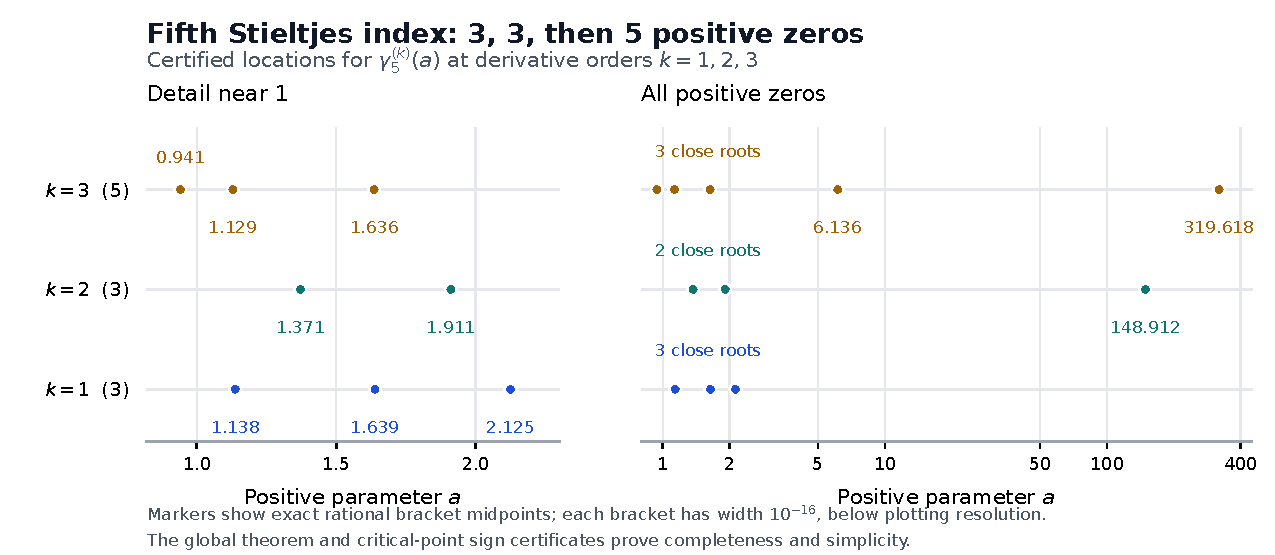
\includegraphics[width=\textwidth]{figures/n5_certified_zero_locations.pdf}
\caption{The eleven certified zero locations. The local panel separates the near-unit roots; the logarithmic panel includes the large roots. The brackets have width $10^{-16}$, much smaller than a plotted marker.}
\label{fig:n5-locations}
\end{figure}

This proof uses no claim that a dense set of sampled values accounts for
every zero.  Completeness at the highest checked order comes from a
global analytic theorem; completeness at lower orders comes from the
complete list of stationary points and their certified signs.

\subsection{Rational Euler--Maclaurin verification}

The certificate is self-contained in
\texttt{certify\_n5\_zeros.py}.  It uses only Python's standard-library
integer and rational arithmetic.  Its output
\texttt{n5\_zero\_certificates.json} records all integer endpoints,
the analytic error bounds, and the assertions that the relevant
intervals exclude zero.  The following derivation specifies its
mathematical contract.

Define exact rational coefficients by
\[
 \prod_{j=1}^{r}(1+z/j)=\sum_i e_i(r)z^i,
 \qquad
 R_{n,r}(v)=n!\sum_{i=0}^{\min(n,r)}
                  e_i(r)\frac{(-v)^{n-i}}{(n-i)!}.
\]
The spectral representation is
\begin{equation}\label{n5:eq:spectral}
 V_{n,k}(a):=\frac{a^{k+1}U_{n,k}(a)}{k!}
   =\sum_{m\geq0}\left(\frac a{a+m}\right)^{k+1}
             R_{n,k}(\log(a+m)).
\end{equation}
In the three orders used here,
\begin{align*}
 R_{5,1}(v)&=-v^5+5v^4,\\
 R_{5,2}(v)&=-v^5+\frac{15}{2}v^4-10v^3,\\
 R_{5,3}(v)&=-v^5+\frac{55}{6}v^4-20v^3+10v^2.
\end{align*}
Higher $r$ in the error analysis use the same exact recurrence, without
numerically evaluating zeta or gamma functions.

For positive rational $a$, choose integers $M,R\geq1$, put $p=k+1$,
$A=a+M>1$, $v=\log A$, and $L=k+2R$.  Set
\begin{align}
 E_{M,R}={}&\sum_{m=0}^{M-1}
       \left(\frac a{a+m}\right)^pR_{n,k}(\log(a+m))\notag\\
 &+\left(\frac aA\right)^p
       \left[\frac Ak R_{n,k-1}(v)+\frac12R_{n,k}(v)\right]\notag\\
 &+\left(\frac aA\right)^p\sum_{r=1}^{R}
    \frac{B_{2r}}{(2r)!}\frac{(k+1)_{2r-1}}{A^{2r-1}}
       R_{n,k+2r-1}(v),\label{n5:eq:EM}
\end{align}
where $(b)_j$ is the rising factorial.  Then
\begin{align}
 |V_{n,k}(a)-E_{M,R}|&\leq
 \left(\frac aA\right)^p\frac{|B_{2R}|}{(2R)!}
       \frac{(k+1)_{2R-1}}{A^{2R-1}}\,\mathcal B_{n,L}(v),
       \label{n5:eq:EM-error}\\
 \mathcal B_{n,L}(v)&=
 \sum_{i=0}^{\min(n,L)}\sum_{j=0}^{n-i}
       \frac{n!e_i(L)}{(n-i-j)!L^j}v^{n-i-j}.
       \label{n5:eq:EM-majorant}
\end{align}
Every factor in the latter bound is nonnegative.

For clarity, the periodic-Bernoulli error estimate in
\eqref{n5:eq:EM-error} is sufficient; no first-omitted-term sign assertion
is needed.  With
$f(x)=x^{-k-1}R_{n,k}(\log x)$, direct coefficient differentiation gives
\[
 f^{(q)}(x)=(-1)^q(k+1)_q x^{-k-q-1}
                            R_{n,k+q}(\log x).
\]
The integral of $f$ from $A$ to infinity is
$A^{-k}R_{n,k-1}(\log A)/k$, which produces the integral term in
\eqref{n5:eq:EM}.  Euler--Maclaurin through the $R$th Bernoulli
correction gives the remaining terms.  Its remainder is bounded by
$|B_{2R}|/(2R)!$ times $a^{k+1}\int_A^\infty|f^{(2R)}(x)|\,dx$.
Majorize $R_{n,L}$ by its coefficientwise absolute values at
$\log x>0$ and use
\[
 \int_A^\infty x^{-L-1}\log^d x\,dx
  =\frac{A^{-L}}{L}
        \sum_{j=0}^{d}\frac{d!}{(d-j)!L^j}\log^{d-j}A.
\]
The leading $L$ cancels the last factor of $(k+1)_{2R}$, yielding
exactly \eqref{n5:eq:EM-error}--\eqref{n5:eq:EM-majorant}.

For logarithms, reduce a positive rational argument to $2^b y$ with
$1\leq y<2$, set $u=(y-1)/(y+1)$, and use
\begin{equation}\label{n5:eq:log-error}
 0\leq\log y-2\sum_{j=0}^{T-1}\frac{u^{2j+1}}{2j+1}
 \leq\frac{2u^{2T+1}}{(2T+1)(1-u^2)}.
\end{equation}
The same formula with $y=2$ encloses $\log2$.  Exact rational
Bernoulli numbers come from their finite triangular recurrence, while
the $e_i(r)$ come from multiplying the finite products above.

The executed parameters are
\[
       n=5,\quad M=24,\quad R=16,\quad T=120,
       \qquad\hbox{fixed denominator }10^{80}.
\]
Every addition, multiplication, division, and integer power is rounded
outwards at this denominator.  The largest analytic
Euler--Maclaurin error bound among all thirty enclosures is less than
$2.591\times10^{-32}$.  This statement concerns the analytic truncation
error; the separate rational interval widths also include all arithmetic
rounding and, where appropriate, the uncertainty across a root bracket.
The final signs are proved by the complete intervals, not by comparing
only the analytic error with a floating-point value.

The code checks twenty-two endpoint signs and eight uniform
critical-point signs.  Evaluating the same interval formulas with
$a$ ranging over a rational interval remains valid by ordinary interval
arithmetic and monotonicity of the logarithm.  This is how
Table~\ref{n5:tab:critical} certifies values at roots without assigning
an exact value to a numerical approximation.

\subsection{Consequences and further questions}

The baseline correctly limited its all-order small-index theorem to
$n\leq4$.  The new fifth-index theorem therefore resolves its first
explicitly open small-order case, rather than correcting a theorem
already stated with the necessary restriction.  It rules out extending
the conclusion to all $n$ at every $k\geq1$.

Several precise continuation questions now replace that false
extrapolation.  Determine the classical saturation threshold
\[
 K_n^{\mathrm{cl}}=
   \min\{k\geq1:N_{n,k}=n\text{ and all positive zeros are simple}\}.
\]
The present results give $K_n^{\mathrm{cl}}=1$ for $1\leq n\leq4$
and $K_5^{\mathrm{cl}}=3$.  Monotonicity and parity constrain every
possible count sequence, while the concentration theorem guarantees an
eventual threshold at each fixed index.  An effective upper bound in
terms of the extreme Appell-root spacing would turn this qualitative
fact into a terminating certified search.

The descending critical-value method applies beyond the fifth index:
once one derivative order is globally saturated and its roots are
isolated, uniform enclosures of the preceding derivative at those
critical points determine the complete lower-order zero count.  It is
particularly useful when the positive roots span several orders of
magnitude.  The count sequence need not increase at every step; the
plateau $3,3$ followed by $5$ is already an exact example.

Finally, quantify how the additional classical zeros arise as the Lerch
parameter increases from zero to one.  The lower bound in
Proposition~\ref{n5:prop:lower} uses exact unit-shift endpoint identities
at the classical endpoint and does not hold for arbitrary $\rho<1$.
This gives a structural reason to study branch creation as well as the
motion of existing simple zeros.

\section{Small positive Lerch parameters and real-zero bifurcations}
\label{sec:lerch}
The uniform eventual-zero theorem in the baseline holds with the Laurent
index fixed and the derivative order sufficiently large. At a fixed small
derivative order, the deformation parameter has a substantially different
effect. A multiple real zero at the elementary endpoint can split into
nonreal zeros, and real branches that do exist can move in opposite
directions. We give an exact classification near that endpoint.

\subsection{An elementary polynomial controls the splitting}
For integers $n\ge1$, $k\ge1$, set
\begin{equation}\label{eq:lerch-h}
 h_{n,k}(a)=\frac{d^k}{da^k}\frac{\log^n a}{a},\qquad
 D_{n,k}^{\rho}(a)=\sum_{m=0}^{\infty}\rho^m h_{n,k}(a+m)
 \quad(0\le\rho\le1).
\end{equation}
At $\rho=1$ this is $\gamma_n^{(k)}(a)$. The series in
\eqref{eq:lerch-h} converges absolutely even there because $k\ge1$.
For $\rho<1$ it is the $k$th parameter derivative of
$(-1)^n\partial_s^n\Phi(\rho,s,a)|_{s=1}$, so it agrees with the
Lerch family used in the manuscript. The underlying Lerch series and
Mellin integral are classical \cite{DLMFLerch,Coffey}.

Define integer polynomials $\mathscr R_{n,k}$ by
\begin{equation}\label{eq:R-recurrence}
 \mathscr R_{n,0}(x)=x^n,\qquad
 \mathscr R_{n,k+1}(x)=\mathscr R_{n,k}'(x)-(k+1)\mathscr R_{n,k}(x).
\end{equation}
Repeated differentiation gives the exact identity
\begin{equation}\label{eq:R-identity}
 h_{n,k}(a)=a^{-k-1}\mathscr R_{n,k}(\log a).
\end{equation}
This recurrence is an efficient way to decide the finite sign appearing
in the theorem below; no evaluation of a special function is needed.

\begin{lemma}\label{lem:elementary-roots}
If $n>k$, then $h_{n,k}$ has a zero of multiplicity $r=n-k$ at $a=1$
and exactly $k$ further positive zeros, all simple and greater than $1$.
If $n\le k$, all its $n$ positive zeros are simple and greater than $1$.
Moreover $h_{n,k}(2)\ne0$ for all $n,k\ge1$.
\end{lemma}
\begin{proof}
Put
\[
 P_{n,k}(x)=\prod_{j=1}^{k}(1+\partial_x/j)x^n.
\]
Then $h_{n,k}(a)=(-1)^{n+k}k!a^{-k-1}P_{n,k}(-\log a)$.
For a real-rooted polynomial $p$, the equation
$p'/p=-1/c$ shows that $p+cp'$ with $c>0$ has one simple
root in each gap between the distinct roots, one simple exterior root,
and only the inherited multiple roots, each with its multiplicity reduced
by one. Starting from $x^n$, after $k<n$ operations the root $0$ has
multiplicity $n-k$ and all $k$ other roots are simple. Every coefficient
of $P_{n,k}$ is nonnegative, and its nonzero coefficients have consecutive
degrees. Thus none of its nonzero real roots is positive. After the
$k=n$ step the constant coefficient is positive; all roots are then
strictly negative and simple, and later steps preserve these properties.
This proves the zero assertions after $a=e^{-x}$.

The polynomial $\mathscr R_{n,k}$ is nonzero with integer coefficients. If
$\mathscr R_{n,k}(\log2)$ vanished, $\log2$ would be algebraic, contrary to the
Hermite--Lindemann theorem \cite{Baker}. Equivalently, the nontrivial
zeros of $h_{n,k}$ are exponentials of nonzero algebraic numbers and
cannot equal the algebraic number $2$.
\end{proof}

\begin{theorem}[Complete small-parameter zero count]
\label{thm:small-rho}
Fix $n,k\ge1$. If $k\ge n-1$, then, for every sufficiently small
$\rho>0$, $D_{n,k}^{\rho}$ has exactly $n$ positive zeros, all simple.
If $k<n-1$, write $r=n-k\ge2$ and $H=h_{n,k}(2)\ne0$. For every
sufficiently small $\rho>0$, all positive zeros are simple and their
number is
\begin{equation}\label{eq:small-count}
 N_{n,k}(\rho)=
 \begin{cases}
 k+1,&r\text{ odd},\\
 k+2,&r\text{ even and }H<0,\\
 k,&r\text{ even and }H>0.
 \end{cases}
\end{equation}
More precisely, when $k<n$ put $r=n-k$. Near $a=1$, all $r$ complex zeros can be written as
convergent series in $\varepsilon=\rho^{1/r}$, with leading terms
\begin{equation}\label{eq:puiseux}
 a_\omega(\rho)=1+\omega\rho^{1/r}+O(\rho^{2/r}),\qquad
 \omega^r=-\frac{r!}{n!}\,h_{n,k}(2).
\end{equation}
Every other zero $\alpha>1$ of $h_{n,k}$ continues analytically as
\begin{equation}\label{eq:simple-zero-shift}
 \alpha(\rho)=\alpha-
 \frac{h_{n,k}(\alpha+1)}{h_{n,k}'(\alpha)}\rho+O(\rho^2).
\end{equation}
The phrase ``sufficiently small'' may depend on $n,k$; the theorem does
not assert a uniform quantitative threshold as those indices grow.
\end{theorem}
\begin{proof}
First suppose $k<n$ and put $r=n-k$. On a complex disk $|a-1|<\delta<1$, all logarithms in the series have
a consistent principal branch and the series is jointly analytic in
$(a,\rho)$ for $|\rho|<1$. With $a=1+z$, Taylor expansion gives
\begin{equation}\label{eq:local-unfolding}
 D_{n,k}^{\rho}(1+z)
 =\frac{n!}{r!}z^r+O(z^{r+1})+
     \rho\{h_{n,k}(2)+O(z)\}+O(\rho^2).
\end{equation}
For $r\ge1$, substitute $z=\varepsilon u$, $\rho=\varepsilon^r$
and divide by $\varepsilon^r$. The result extends analytically to
$\varepsilon=0$ and equals $(n!/r!)u^r+H$ there. Its $r$ roots are
simple by $H\ne0$. The analytic implicit-function theorem gives $r$
distinct analytic functions of $\varepsilon$, and Rouch\'e's theorem
on a fixed small disk around $a=1$ shows that these account for all
nearby zeros. For positive real $\varepsilon$, a simple real limiting
root gives a real branch by conjugation and uniqueness; a nonreal
limiting root stays nonreal. Counting the real roots of
$(n!/r!)u^r+H$ gives \eqref{eq:small-count}. When $r=1$ the same
argument gives a single real simple continuation. When $k\ge n$ there
is no multiple root to analyze. The other $k$ (or $n$) zeros are handled
by the ordinary analytic implicit-function theorem, which also gives
\eqref{eq:simple-zero-shift}.

It remains to exclude positive zeros that escape these neighborhoods.
This is a global, not just local, step. On $[1,\infty)$, $h_{n,k}$ and
all its fixed derivatives are bounded. Therefore
\[
 \sup_{a>0}\left|\sum_{m\ge1}\rho^m h_{n,k}(a+m)\right|
 \le M_{n,k}\frac{\rho}{1-\rho}.
\]
Near $a=0$, the unperturbed term has fixed sign and unbounded magnitude,
so a sufficiently small fixed neighborhood of zero remains zero-free.
Beyond the largest unperturbed zero, every summand has the same strict
sign, except for the possible vanishing of the first summand at the
endpoint. Hence no zero can escape to infinity. On the remaining compact
set away from the chosen zero neighborhoods, $|h_{n,k}|$ has a positive
minimum and the displayed uniform bound applies. These three regions
exclude every additional positive zero.
\end{proof}

\begin{corollary}[First derivatives collapse to one or two zeros]
\label{cor:first-lerch}
For each fixed odd $n\ge3$, $D_{n,1}^{\rho}$ has exactly one positive
zero for every sufficiently small $\rho>0$. For each fixed even $n\ge2$
it has exactly two. In the even case the smaller zero satisfies
\begin{equation}\label{eq:even-small-root}
 a_-(\rho)=1-
 \left(\frac{(\log2)^{n-1}(n-\log2)}{4n}\right)^{1/(n-1)}
 \rho^{1/(n-1)}+O(\rho^{2/(n-1)}).
\end{equation}
In both cases the large zero tends to $e^n$.
\end{corollary}
\begin{proof}
Here
$h_{n,1}(a)=a^{-2}\log^{n-1}a\,(n-\log a)$, so
$h_{n,1}(2)>0$ and $r=n-1$. Apply Theorem~\ref{thm:small-rho}.
\end{proof}

\begin{table}[htbp]
\centering\small
\begin{tabular}{c|rrrrrrr}
\toprule
$n\backslash k$&1&2&3&4&5&6&7\\\midrule
2&2&2&2&2&2&2&2\\
3&1&3&3&3&3&3&3\\
4&2&2&4&4&4&4&4\\
5&1&3&3&5&5&5&5\\
6&2&2&4&6&6&6&6\\
7&1&3&3&5&7&7&7\\
8&2&2&4&4&6&6&8\\
\bottomrule
\end{tabular}
\caption{The number of positive zeros for sufficiently small positive
$\rho$, with $n,k$ fixed. All signs needed for this table, and the extended
table through $n=16$, are certified using rational bounds on $\log2$.
This table concerns the Lerch endpoint regime, not the classical endpoint
$\rho=1$.}
\label{tab:small-rho}
\end{table}

\subsection{Alternating motion of odd-index first-derivative zeros}
The eventual large-$k$ offset in the baseline decreases with $\rho$ at
every fixed zero label. That asymptotic fact does not extend to all
small derivative orders. The following exact inequality resolves the
issue for odd-index first derivatives.

\begin{theorem}[Direction of motion at every real zero]
\label{thm:rho-direction}
Let $n\ge1$ be odd, $0<\rho<1$, and $D(a,\rho)=D_{n,1}^{\rho}(a)$.
Then every positive zero lies below $e^n$, and
\begin{equation}\label{eq:rho-negative}
 \partial_\rho D(a,\rho)<0\quad\text{whenever }D(a,\rho)=0.
\end{equation}
For each fixed $a>0$, there is at most one zero in the parameter
$0<\rho<1$. On any parameter interval with exactly $N$ positive
simple zeros, numbered increasingly, their motion alternates:
\begin{equation}\label{eq:alternating-motion}
 \frac{d a_j}{d\rho}<0\quad(j\text{ odd}),\qquad
 \frac{d a_j}{d\rho}>0\quad(j\text{ even}).
\end{equation}
Here $N$ is necessarily odd.
\end{theorem}
\begin{proof}
Since $n-1$ is even, $h_{n,1}(t)$ is positive for $0<t<e^n$,
apart from its zero at $t=1$ when $n>1$, and negative for $t>e^n$.
Thus no zero is possible for $a\ge e^n$ when $\rho>0$.
Put $\lambda=e^n-a$. For every $a>0$ and $0<\rho<1$, termwise
differentiation gives the strict inequality
\begin{equation}\label{eq:weighted-rho}
 \rho\partial_\rho D(a,\rho)-\lambda D(a,\rho)
 =\sum_{m\ge0}(m-\lambda)\rho^m h_{n,1}(a+m)<0.
\end{equation}
Every summand is nonpositive: the factors $m-\lambda$ and
$n-\log(a+m)$ have opposite signs. Some summands are strictly
negative, and the series converges absolutely. At a zero this proves
\eqref{eq:rho-negative}. More generally,
$\partial_\rho(\rho^{-\lambda}D)<0$, which proves that there is
at most one parameter zero for each fixed $a$.

The function is positive near $a=0$ and negative for $a\ge e^n$.
Simple real zeros therefore cross with $\partial_aD<0$ at the odd
labels and $\partial_aD>0$ at the even labels. Implicit
differentiation gives $a_j'=-\partial_\rho D/\partial_aD$ and the
claimed signs. This argument only asserts differentiability for
$\rho<1$; it makes no endpoint regularity assumption at $\rho=1$.
\end{proof}

\begin{corollary}[An increasing middle branch]
\label{cor:increasing-middle}
For $n=3$, $k=1$, there is a number $\rho_0<1$ such that for
$\rho_0<\rho<1$ the three positive simple zeros satisfy
\[
 a_1'(\rho)<0,\qquad a_2'(\rho)>0,\qquad a_3'(\rho)<0.
\]
Consequently the proposal that all higher branches decrease with $\rho$
at every derivative order is false. The fixed-index, large-derivative
asymptotic statement in the baseline remains valid.
\end{corollary}
\begin{proof}
At $\rho=1$, the classical $n=3$ function has exactly three positive
simple zeros; an analytic proof is given in Section~\ref{sec:classical-zeros}.
Uniform convergence of \eqref{eq:lerch-h} and its $a$ derivative on
compact positive intervals as $\rho\uparrow1$ preserves opposite
endpoint signs in three disjoint isolating intervals. The global bound
of three zeros counted with multiplicity makes these the only zeros
and makes them simple. Apply Theorem~\ref{thm:rho-direction}.
\end{proof}

\subsection{A nondegenerate creation of two real zeros}
The following endpoint signs, consistent with the baseline small-index certificates, are verified afresh by the rational checker in this package:
\[
 D_{3,1}^1(4/5)>0,\qquad D_{3,1}^1(11/10)<0,\qquad
 D_{3,1}^1(3/2)>0.
\]
These three signs are also recomputed in the present package. They
suffice to make the bifurcation statement fully analytic.

\begin{theorem}[A real saddle-node in the Lerch deformation]
\label{thm:fold}
There are $0<\rho_*<1$ and $4/5<a_*<3/2$ such that
\[
 D_{3,1}^{\rho_*}(a_*)=\partial_aD_{3,1}^{\rho_*}(a_*)=0,
 \quad \partial_a^2D_{3,1}^{\rho_*}(a_*)>0,
 \quad \partial_\rho D_{3,1}^{\rho_*}(a_*)<0.
\]
This is the first parameter at which a zero occurs in $[4/5,3/2]$;
there is only one double zero there at that parameter. For every
$\rho_*<\rho<1$, the interval contains exactly two simple zeros and
there is exactly one further positive zero. Near $\rho_*$ the two
zeros have the expansions
\begin{equation}\label{eq:fold-expansion}
 a_\pm(\rho)=a_*\pm
 \sqrt{-\frac{2\partial_\rho D(a_*,\rho_*)}
                  {\partial_a^2D(a_*,\rho_*)}}
       \sqrt{\rho-\rho_*}+O(\rho-\rho_*).
\end{equation}
The smaller branch decreases and the middle branch increases throughout
$(\rho_*,1)$.
\end{theorem}
\begin{proof}
For a fixed $a$, \eqref{eq:weighted-rho} shows that a negative value,
once reached as $\rho$ increases, remains negative. Since the two
endpoint values are positive at $\rho=1$, they are positive for every
$0<\rho<1$. Corollary~\ref{cor:first-lerch} and its proof show that
$D$ is strictly positive on the whole interval $[4/5,3/2]$ for all
sufficiently small positive $\rho$. The negative value at $11/10$ for
$\rho=1$ persists for parameters sufficiently close to one. Compactness
and continuity therefore give a first parameter $\rho_*\in(0,1)$
where the minimum on the interval is zero. More explicitly, take
\[
 \rho_*=\inf\{0<\rho<1:\min_{a\in[4/5,3/2]}D(a,\rho)\le0\}.
\]
The restriction $\rho>0$ excludes the multiple zero of the elementary endpoint itself. The preceding small-parameter positivity keeps this infimum away from zero. That minimum is attained
at an interior point $a_*$, where $D=\partial_aD=0$.

For every $0<\rho<1$, positivity at $3/2$ and negativity at $e^3$
force a further sign-changing zero in $(3/2,e^3)$. At $\rho_*$,
the double-or-higher zero in $[4/5,3/2]$ together with that further
zero uses at least three units of multiplicity. The global bound of
three therefore makes the first zero exactly double, makes it unique
in the first interval, and excludes every additional zero. Since it
is a local minimum, $\partial_a^2D>0$. Equation~\eqref{eq:rho-negative}
gives $\partial_\rho D<0$.

For every $\rho>\rho_*$, the value at the fixed point $a_*$ is
negative. The positive endpoints give two distinct zeros in the
interval, and the right-hand sign change gives a third. The global
bound makes all three simple and excludes others. Their directions
follow from Theorem~\ref{thm:rho-direction}. Finally the analytic
Taylor expansion at the double zero, or the implicit-function theorem
applied with $\sqrt{\rho-\rho_*}$ as local parameter, gives
\eqref{eq:fold-expansion}.
\end{proof}

The supplied quadrature diagnostic locates the fold and illustrates the
square-root law. Those decimal estimates are not used to prove the
bifurcation, its nondegeneracy, or the direction of the middle branch.
The theorem does not claim that no other changes in the rightmost
zero configuration occur below $\rho_*$; a complete classification of
that earlier parameter interval is a separate question.

\section{Corrections, conjectures, and further research}
\label{sec:research-program}

\subsection{Two precise corrections to the pinned text}

\paragraph{A consequence is not an equivalence.}
In \texttt{05-signed-kernels.tex}, immediately after
\texttt{signed:eq:rank-conjecture}, the manuscript calls the pair of rank
formulas equivalent to a statement about the dimension of the
Gaussian-supported row space. If $V_w$ is the row space, projection onto
the non-Gaussian columns gives exactly
\[
 \dim\bigl(V_w\cap\QQ^{\{g\text{-columns}\}}\bigr)
 =\rank A_w-\rank A_w^{\neg g}.
\]
Thus the two individual ranks imply the stated dimension, while their
difference alone does not determine either individual rank. Replace
``Equivalently'' by ``Consequently,'' and replace the following sentence
about the equivalence by a sentence about this dimension formula.
Theorem~\ref{newrank:thm:smith} now proves both ranks, so the conjecture can
also be promoted to a theorem when its proof is integrated. The companion
patch makes the narrow logical correction without assuming a particular
chapter-insertion scheme.

\paragraph{Even modified polylogarithms on real arguments.}
In \texttt{03-algebraic.tex}, equation \texttt{bloch:eq:Pm} defines
\[
 P_m(x)=\operatorname{Re}_m\left(
       \sum_{j=0}^{m-1}\frac{2^jB_j}{j!}\log^j|x|\,\Li_{m-j}(x)
       \right),\qquad
 \operatorname{Re}_m=
 \begin{cases}\Re,&m\text{ odd},\\\Im,&m\text{ even}.
 \end{cases}
\]
The later paragraph on higher golden ladders says that the same
coordinates turn a real weight-six ladder into a $\zeta(6)$ multiple.
With this definition, $P_6$ is identically zero on real arguments.
The text itself correctly states this parity fact a little later. In
particular, for the golden arguments in $(0,1)$ every summand inside the
imaginary part is visibly real. A nonzero multiple of $\zeta(6)$ cannot
be the value of that real-argument modified-polylogarithm combination.

The correction is local: remove the weight-six assertion in these
coordinates, retain the raw classical-polylogarithm identity at whatever
status its independent evidence supports, and check odd-weight conversions
directly from the definition. The supplied replacement text avoids
asserting unverified conversions at the other higher weights. No claim
that the raw weight-six ladder is false follows from this observation.

\subsection{Statements that require qualification, not retraction}

The fifth-index theorem does not contradict the baseline theorem, whose
small-index conclusion is restricted to $n\le4$. It disproves the
unrestricted extrapolation of that conclusion. Similarly, the increasing
middle Lerch branch does not contradict a large-derivative asymptotic
offset formula. It shows that its monotonic direction cannot be imposed
on every branch at every small derivative order.

The CM product theorem is a norm statement unless a phase is supplied.
The real-part convention at discriminant $-15$ is mathematically material:
the factor $7/8$ cannot be omitted. The absolute norm alone does not
license a raw signed product at arbitrary discriminants or weights.

The weight-five witness proves an obstruction only for the specified
linear product matrix. No period-independence claim, no impossibility of
using higher-depth relations, and no negative answer to the $S_4$
conjecture follows. This scope was already correctly emphasized by the
baseline; the shorter integral witness makes it easier to check.

\subsection{A concrete next zero-count conjecture}

\begin{conjecture}[Sixth- and seventh-index first derivatives]
\label{conj:n6n7}
The function $\gamma_6'$ has exactly four positive zeros and
$\gamma_7'$ has exactly five positive zeros. In each case every positive
zero is simple.
\end{conjecture}

The numerical candidates are
\begin{align*}
 n=6:\quad&0.8426787120,\ 1.2904536569,\ 1.7994089556,\ 2.2385946523;\\
 n=7:\quad&0.7781418150,\ 0.9499243123,\ 1.4420456198,\\
           &1.9499308927,\ 2.3354109288.
\end{align*}
These statements are \emph{conjectures}, not further certified theorems.
The supplied diagnostic uses 70 decimal digits, an Euler--Maclaurin
evaluation with $M=24$, $R=16$, and 992 test points at each index: 401
logarithmic points spanning $10^{-3}$ to $10^{3.1}$ and 591 linear points
$j/200$, $60\le j\le650$. Root refinement produces the displayed values.
At first derivative order the spectral summands are negative once
$a>e^n$, so this upper tail is analytically free of zeros. Nevertheless,
the finite scan does not certify the unsampled intervals or exclude a
tangency. A proof should use global saturation at a higher derivative
order and descend through every critical point, as in
Theorem~\ref{n5:thm:transition}.

The conjecture is deliberately finite. These two observations do not
support a simple universal formula for the first-derivative count:
the oscillation near $a=1$, the wide range of large roots at higher
derivative orders, and the count plateaus already proved at index five
make extrapolation hazardous.

\subsection{A focused program for the formal relation system}

\paragraph{Construct certificates without elimination.}
The proof of Theorem~\ref{newrank:thm:smith} identifies a unimodular
coordinate system in which the problem breaks into one- and two-variable
blocks. Turn that proof into an explicit symbolic certificate compiler.
For a target vector, it should either return an integer row combination
(or, in even weight, one for twice the target) or return an integral
annihilating witness. The witness basis is already explicit, so membership
testing can be performed with only $w-1$ pairings in odd weight. Tracking
the affine right sides through the same transformations is the remaining
engineering and symbolic-algebra task.

\paragraph{Identify the missing relation for $S_4$.}
The six-entry witness pairs to $7$ with the target. Any proposed
enlargement must include a relation whose coefficient vector does not
annihilate that witness. This provides an exact preliminary test before
computing a much larger matrix. Candidates include distribution,
argument transformations, and elimination through higher depth. The
research question is not merely whether an enlarged matrix has larger
rank, but which analytically justified relation kills this particular
obstruction and with what right side.

\paragraph{Determine the effect of distribution integrally.}
The $2$-torsion in even weight is a property of the stated product
presentation. Does adjoining the appropriate distribution rows remove
some or all of it? What is the Smith form of that enlarged lattice?
This is a concrete question about an explicitly constructible sequence of
integer modules; no unproved transcendence assumption is required.

\paragraph{Generalize the involution method to other levels.}
At level four, conjugation reduces the colors to six and the residual
action becomes the swap $(u,v)\mapsto(v,u)$. At other small levels,
determine whether an integral color decomposition produces similarly
manageable finite-group actions on homogeneous polynomials. Rational
rank formulas alone would miss torsion introduced by nonunimodular
changes of basis, so an integral formulation should be maintained from
the outset.

\subsection{A focused program for CM identities}

\paragraph{Automate the exact arithmetic factor.}
For fixed even weight, generate $F_w$ in exact rational arithmetic and
evaluate its resultant with a certified Hilbert class polynomial.
At weights four and six the arithmetic is concentrated in
$H_D(0)$ and $H_D(1728)$; in higher weights the zeros of the Eisenstein
series create additional algebraic factors. A systematic collection of
these factors would distinguish patterns forced by modular algebra from
patterns inferred from decimal recognition.

\paragraph{Classify phases and genus refinements.}
Extend the phase analysis along the unit arc to every even weight,
including the additional arc zeros of $E_w$. Extend the proved character
products to nonmaximal orders and combine several independent genus
characters to recover every genus product. For higher genus rank the
plus and minus fibers of one character are unions of genera. These are the natural intermediate
objects between a full class norm and an individual CM evaluation.
Every claimed formula should specify the reduced representative,
automorphy factor, and chosen algebraic embedding.

\paragraph{Move beyond full norms.}
For larger class groups, determine individual algebraic factors relative
to a fixed CM period. For the genus ratios, determine when the uniform
degree bound of Theorem~\ref{cmgenus:thm:degree} is attained, and which
proper subfields occur as the weight changes. A rational class norm does not imply that raw sums of
positive-weight CM values are rational or Galois-invariant. Replacing
such raw sums by explicitly normalized modular quantities is the natural
route to well-posed algebraicity questions.

\subsection{A focused program for zero geometry}

\paragraph{Determine saturation thresholds.}
Set
\[
 K_n^{\mathrm{cl}}=\min\{k\ge1:\gamma_n^{(k)}
       \text{ has }n\text{ positive simple zeros}\}.
\]
The exact values are now $K_n^{\mathrm{cl}}=1$ for $1\le n\le4$ and
$K_5^{\mathrm{cl}}=3$. The baseline concentration theorem implies that
the threshold exists for every fixed index. Find a useful effective
bound in $n$, and then determine whether the sequence of thresholds has
any monotonicity or regular asymptotic behavior. The proved parity and
count monotonicity restrict possible answers but do not determine them.

\paragraph{Make the small-parameter theorem effective.}
Theorem~\ref{thm:small-rho} gives a complete count for sufficiently small
positive $\rho$, but not an explicit threshold. Its proof suggests a
constructive route: isolate the algebraic roots of the integer
polynomial, bound derivatives on disjoint disks, and bound the remaining
series uniformly. Quantifying the separation from $\log2$ is the
sensitive step. Transcendence proves nonvanishing, while a useful
numerical threshold needs an effective separation bound.

\paragraph{Certify the fold coordinates.}
The existence and nondegeneracy of the index-three fold are proved.
The diagnostic predicts
\[
 a_*\approx1.04975305088025546,\qquad
 \rho_*\approx0.999990466837738634.
\]
Produce a rational interval box for this pair by applying an interval
Newton method to $(D,\partial_aD)$, with explicit quadrature or
Euler--Maclaurin remainders in both variables. The determinant of the
Jacobian is $-\partial_\rho D\,\partial_a^2D>0$ at the fold, so the
proved nondegeneracy identifies the right certification problem. The
decimals above are not yet such a box.

\paragraph{Describe the entire deformation, not only its endpoints.}
For odd $n$ at first derivative order,
$\partial_\rho(\rho^{-(e^n-a)}D)<0$. Thus each fixed $a$ changes sign
at most once. Determine the topology of the resulting sign domains:
which negative intervals are created, which can merge, and which
bifurcations are possible under the global multiplicity bound. For
$n=3$, the proved fold controls all parameters after its first appearance
in $[4/5,3/2]$, while the possible earlier configuration on the right
remains a separate question.

\paragraph{Treat the simultaneous large-index regime.}
The baseline concentration expansion fixes $n$ and lets $k$ grow.
The extreme roots of $Q_n$ change with $n$, and the small-parameter
Puiseux exponent $1/(n-k)$ exhibits another nonuniform limit. Determine
which double-scaling regimes preserve the known zero approximations,
and where the right asymptotic description must change. A satisfactory
answer would connect the formal spectral polynomials, reciprocal-gamma
root geometry, and the observed threshold sequence.

\appendix
\section{Reproducibility, evidence boundaries, and integration}
\label{app:reproducibility}

\subsection{What the package contains}

The archive contains the article source, its component sections, the
compiled PDF, vector figures with plotting sources, exact verification
programs, numerical diagnostics, and machine-readable receipts. A
provenance manifest records the pinned source commit and the SHA-256
digests of the consulted manuscript files. A separate claim ledger maps
results to their proofs, their scripts, and their status. The two narrow
text corrections are provided as an ordinary unified patch, together with
integration notes keyed to existing manuscript labels.

The article is a self-contained continuation, not a silent replacement
of the 228-page source manuscript. Each contribution is isolated in a
section file so that a repository maintainer can move it to the relevant
chapter. Numbered labels have distinct prefixes for the relation-lattice,
mixed-family, CM, and classical-zero contributions. The common zero
preliminaries can be omitted when integrating into the existing zero
chapter, provided the references are redirected to its established
theorems.

\subsection{Exact computations and analytic certificates}

\begin{center}
\small
\begin{tabularx}{\textwidth}{@{}>{\raggedright\arraybackslash}p{0.31\textwidth}>{\raggedright\arraybackslash}X>{\raggedright\arraybackslash}p{0.21\textwidth}@{}}
\toprule
Program & Verified object & Logical status\\
\midrule
\texttt{verify\_rank.py} & Integer rows, rational ranks, primitive kernel
witnesses, and Smith forms in the specified finite range. & Exact
algebra; checks the general proof.\\[3pt]
\texttt{verify\_mixed\_family.py} & A finite integer row certificate for
twice the target at even weights; independent integral evaluation. &
Exact rows; quadrature is diagnostic.\\[3pt]
\texttt{cm\_norms.py} & Reduced forms, interval-enclosed singular moduli,
unique integer class-polynomial coefficients, exact factorizations. &
Certified computation using CM integrality.\\[3pt]
\path{cm_genus.py} & Quadratic-field factors, certified genus labels,
and exact cubic and square identities for the ratios. & Exact and interval certificate.\\[3pt]
{\footnotesize\texttt{modular\_weight\_polynomials.py}} & Exact $F_w$ and coefficient
identities through the weight-$12w$ valence bound, $4\le w\le24$. & Exact modular-form certificate.\\[3pt]
\path{certify_n5_zeros.py} & Rational interval signs at all eleven
root brackets and all eight needed critical values; three index-three
endpoint signs. & Finite analytic certificate.\\[3pt]
\path{certify_lerch_splitting.py} & 120 signs of integer polynomials
at $\log2$, for $2\le n\le16$. & Exact rational enclosures.\\[3pt]
\texttt{lerch\_fold\_diagnostic.py} & A high-precision approximate
solution of $D=\partial_aD=0$. & Numerical diagnostic only.\\[3pt]
\texttt{explore\_n6\_n7.py} & Finite scans and root refinements supporting
Conjecture~\ref{conj:n6n7}. & Numerical evidence only.\\
\bottomrule
\end{tabularx}
\end{center}

The zero certificate uses only Python's integer and rational arithmetic;
its logarithm bounds and Euler--Maclaurin remainder are proved in the
text. It does not call a numerical Stieltjes-constant routine. The matrix
certificate uses exact SymPy arithmetic and an independently constructed
matrix. The mixed-family certificate works directly with product rows,
and the all-weight proof supplies the uniform row combination.

The six radical genus evaluations also have an independent checker,
\path{verify_genus_arithmetic.py}, which performs arithmetic as rational
pairs in the two quadratic fields and checks the positive-root choices.
It imports neither SymPy nor the CM verifier.

The CM coefficient certificate uses the directed interval implementation
in \texttt{mpmath.iv}. Its proof contract is explicit: the elementary
interval functions enclose their true values, the rational tail bound is
added before division or multiplication, and each resulting coefficient
interval has a unique possible integer. Classical CM integrality supplies
the fact that the true coefficient is an integer. This is a conventional
computer-assisted proof, with the interval implementation as part of its
trusted computational base. No claim of proof-assistant formalization is
made.

\subsection{Replay and interpretation}

From the extracted archive, the principal commands are
\begin{verbatim}
python3 -m pip install -r requirements.txt
python3 code/verify_all.py
latexmk -pdf -interaction=nonstopmode -halt-on-error article.tex
\end{verbatim}
The replay driver runs each principal verifier in a fresh output
directory, preserving the delivered receipts for comparison. Numerical
diagnostics can be run separately with the documented flag. They are
excluded from the proof-only interpretation even when they agree to the
full working precision.

For the rank replay, the delivered run covers weights $3$ through $13$
and both Smith forms through weight $12$. It checks the $92\times23$
weight-five matrix and the exact pairing $7$ of the short witness with
the target. For the mixed family, the finite row certificate is checked
at all even weights $4$ through $20$, and the independent integral at
weights $2,4,6,8,10$. The general claims are proved in the article;
these finite ranges are validation ranges, not the asserted scope of
the theorems.

The article's PDF was compiled with all cross-references resolved and
rendered for visual inspection. Figure labels, tables, long formulas,
and page breaks were checked. The archive includes a checksum manifest
so that later editorial changes can be distinguished from the delivered
research version.

\subsection{Suggested integration order}

First apply the two local corrections. Next insert the relation-lattice
theorem after the formal product system and replace the old odd-weight
rank conjecture by a reference to the theorem. Place the mixed-family
identity next to the existing Gaussian and signed-color evaluations.
In the CM chapter, upgrade the product identities only after inserting
the period normalization, certified class data, and phase conventions.
In the zero chapter, put the fifth-index transition after the small-index
certificates, and the small-parameter and bifurcation results after the
definition of the Lerch family. Retain the diagnostic labels on the
fold coordinates and the sixth- and seventh-index conjectures.

This integration order preserves the distinction between a theorem,
an exactly checkable finite lemma, an independently verified numerical
identity, and an open conjecture throughout the combined manuscript.

\clearpage
\begingroup
\small
\begin{thebibliography}{99}
\raggedright
\bibitem{ProveIt}
ProveIt Contributors,
\emph{Polylogarithms and their Arithmetic Bridges:
Special Values, Zeta Jets, Lattices and Experimental Discovery},
ProveIt repository, 228-page version at commit
\texttt{9bc738d3be22b8586a24693f19fb2e2a50ecd1bf}, 10 October 2026.
\url{https://github.com/VladimirReshetnikov/ProveIt/tree/9bc738d3be22b8586a24693f19fb2e2a50ecd1bf/Analysis/Polylogarithms/docs/manuscript}.

\bibitem{Zhao}
J.~Zhao, \emph{Standard relations of multiple polylogarithm values at
roots of unity}, Documenta Mathematica \textbf{15} (2010), 1--34.
\url{https://ems.press/journals/dm/articles/8965225}.

\bibitem{YuanZhao}
H.~Yuan and J.~Zhao, \emph{Double shuffle relations of double zeta
values and double Eisenstein series of level $N$}, Journal of the London
Mathematical Society \textbf{92} (2015), 520--546.
\url{https://arxiv.org/abs/1401.6699}.

\bibitem{DLMFLerch}
NIST Digital Library of Mathematical Functions, Section 25.14,
\emph{Lerch's transcendent}.
\url{https://dlmf.nist.gov/25.14} (accessed 10 October 2026).

\bibitem{DLMFHurwitz}
NIST Digital Library of Mathematical Functions, Section 25.11,
\emph{Hurwitz zeta function}.
\url{https://dlmf.nist.gov/25.11} (accessed 10 October 2026).

\bibitem{DLMFGamma}
NIST Digital Library of Mathematical Functions, Section 5.8,
\emph{Infinite products for the gamma function}.
\url{https://dlmf.nist.gov/5.8} (accessed 10 October 2026).

\bibitem{Coffey}
M.~W.~Coffey, \emph{Series representations for the Stieltjes constants},
Rocky Mountain Journal of Mathematics \textbf{44} (2014), 443--477.
\url{https://arxiv.org/abs/0905.1111}.

\bibitem{Baker}
A.~Baker, \emph{Transcendence theory and its applications},
Journal of the Australian Mathematical Society, Series A
\textbf{25} (1978), 438--444.
\href{https://doi.org/10.1017/S144678870002142X}{doi:10.1017/S144678870002142X}.
Section 3 recalls the Hermite--Lindemann theorem used for
$\log2\notin\overline{\QQ}$.

% Insert these items inside the article's thebibliography environment.
\bibitem{cmnorm:Barquero}
A.~Barquero-Sanchez, L.~Cadwallader, O.~Cannon, T.~Genao, and R.~Masri,
\emph{Faltings heights of CM elliptic curves and special Gamma values},
Research in Number Theory \textbf{3} (2017), article 13.
\href{https://doi.org/10.1007/s40993-017-0077-7}{doi:10.1007/s40993-017-0077-7}.
Sections 3--5 give the analytic normalization of the Kronecker and
Chowla--Selberg formulas, including nonmaximal quadratic orders.

\bibitem{cmnorm:Cohen2026}
H.~Cohen, \emph{On the Argument of the Lerch, Chowla--Selberg Formula
and CM Values of $\eta(\tau)$}, arXiv:2606.02904v1 (2026).
\url{https://arxiv.org/html/2606.02904v1}.
Theorem 1.3 states the period-product formula with conductor correction;
Theorem 2.1 addresses the choice of representatives and eta phases.

\bibitem{cmnorm:Sutherland}
A.~V.~Sutherland, \emph{Computing Hilbert class polynomials with the
Chinese Remainder Theorem}, Mathematics of Computation \textbf{80}
(2011), 501--538.
\href{https://math.mit.edu/~drew/classpoly.html}{Author's implementation and references}.

\bibitem{cmnorm:YuiZagier}
N.~Yui and D.~Zagier, \emph{On the singular values of Weber modular
functions}, Mathematics of Computation \textbf{66} (1997), 1645--1662.
\href{https://people.mpim-bonn.mpg.de/zagier/files/doi/10.1090/S0025-5718-97-00854-5/fulltext.pdf}{Author-hosted full text}.


\bibitem{Stein}
W.~Stein, \emph{Modular Forms: A Computational Approach},
Graduate Studies in Mathematics, vol.~79, American Mathematical Society, 2007.
Author-hosted text, Chapter 2 (level-one structure and valence formula).
\url{https://wstein.org/books/modform/modform/level_one.html}.

\bibitem{cmgenus:MurtyMurty}
M.~Ram Murty and V.~Kumar Murty,
\emph{Transcendental values of class group $L$-functions},
Mathematische Annalen \textbf{351} (2011), 835--855,
Section~5 (Kronecker's genus-character factorization),
\url{https://doi.org/10.1007/s00208-010-0619-y}.

\bibitem{cmgenus:Masri}
R.~Masri,
\emph{Kronecker's solution of Pell's equation for CM fields},
Annales de l'Institut Fourier \textbf{63} (2013), 2287--2306,
equations (1.3)--(1.5),
\url{https://doi.org/10.5802/aif.2830}.


\end{thebibliography}
\endgroup
\end{document}
